\documentclass[preprint,10pt,authoryear]{elsarticle}
\pdfoutput=1
\pdfminorversion=4
\usepackage[utf8]{inputenc}
\usepackage[T1]{fontenc}
\usepackage[english]{babel}
\usepackage{amsmath}
\usepackage{multicol}
\usepackage[usenames, dvipsnames]{xcolor}
\usepackage{graphicx}
\usepackage{caption}
\usepackage{subcaption}
\usepackage[margin=1.4in]{geometry}
\usepackage{float}
\usepackage{array}
\usepackage{graphicx}
\usepackage{siunitx}
\graphicspath{{../src/figures/}}
\usepackage{rotating}
\usepackage[labelfont={bf,up}, font={small}]{caption}
\usepackage{sidecap}
\sidecaptionvpos{figure}{c}
\usepackage[colorinlistoftodos]{todonotes}
\usepackage{adjustbox}
\usepackage{placeins}
\usepackage{lineno}
\usepackage{tabularx}
\DeclareUnicodeCharacter{00A0}{~}
\bibliographystyle{elsarticle-harv}
\biboptions{square}

\renewcommand\familydefault{\sfdefault}
\usepackage[scaled]{helvet}

\usepackage{units}


%\usepackage{soul}
\usepackage{soulutf8}
\usepackage{placeins}

\usepackage{nameref}
\usepackage[pdftex,breaklinks=true,colorlinks=true,linkcolor=blue,citecolor=blue,urlcolor=blue,filecolor=blue,pdffitwindow,pagebackref=false,bookmarks=true,bookmarksopen=true,bookmarksnumbered=true]{hyperref}
\usepackage[plain]{fancyref}
\usepackage{array}
\usepackage{multirow}

%custom color for \hlc
\newcommand{\hlb}[2][NavyBlue]{ {\sethlcolor{#1} \hl{#2}} }
\newcommand{\hlg}[2][Emerald]{ {\sethlcolor{#1} \hl{#2}} }
\newcommand{\hlp}[2][Purple]{ {\sethlcolor{#1} \hl{#2}} }


%boxes and highlight color for text updates, personified!
\newcommand{\snnote}[1]{\color{white}{\hlb{SN: #1 }}\color{black}}
\newcommand{\sntxt}[1]{{\color{NavyBlue}#1}}
\newcommand{\tvnnote}[1]{\color{white}{\hlg{TVN: #1 }}\color{black}}
\newcommand{\tvntxt}[1]{{\color{Emerald}#1}}
\newcommand{\gtenote}[1]{\color{white}{\hlp{GTE: #1 }}\color{black}}
\newcommand{\gen}[1]{\color{white}{\hlp{GTE: #1 }}\color{black}}
\newcommand{\gtetxt}[1]{{\color{Orange}#1}}
\newcommand{\gex}[1]{{\color{Orange}#1}}
\usepackage{ulem} % for deleting = strike out


\begin{document}
	
\begin{frontmatter}
	%\linenumbers
	
	\title{Biophysical modeling of the neural origin of EEG and MEG signals
%	\tvnnote{Alternativ tittel: 
%%			1) Towards a model-based understanding of the EEG signals.
%%			2) Towards accurate detailed biophysical modeling of EEG signals.}
	}
	
	\author{Solveig N\ae{}ss\corref{cor1}\fnref{label1}}
	\author{Geir Halnes\fnref{label2}}
	\author{Espen Hagen \fnref{label5}}
	\author{Eric Halgren\fnref{label3}}
	\author{Don Hagler\fnref{label3}}
	\author{Anders M. Dale\fnref{label4}}
	\author{Gaute T. Einevoll\fnref{label2,label5}}
	\author{Torbj\o{}rn V. Ness\fnref{label2}}
	
	\address[label1]{Department of Informatics, University of Oslo, Oslo, Norway}
	\address[label2]{Faculty of Science and Technology, Norwegian University of Life Sciences, Ås, Norway}
	\address[label3]{Department of Radiology, University of California, San Diego, CA, USA}
	\address[label4]{Departments of Neurosciences and Radiology, University of California, San Diego, CA, USA}
	\address[label5]{Department of Physics, University of Oslo, Oslo, Norway}
	%\cortext[cor1]{correspondance: \href{}{}}
	
	%\date{\today}
	
	\begin{abstract}
	\tvnnote{This is not done yet} \gen{Have not looked at this}
		Many important brain signals, like the LFP, ECoG, EEG and MEG are thought to primarily reflect synaptic input to populations of geometrically aligned pyramidal neurons. Therefore, it is important to get a better understanding of the biophysics underlying the synaptic contribution to these brain signals. For a pyramidal neuron receiving a single synaptic input, it is well established that the ensuing extracellular potential will take the shape of a dipole in the far field limit, i.e., sufficiently far away from the neuron. This can potentially greatly simplify the link between the measured brain signals and the underlying neural sources, but this link has not yet been taken full advantage of in the framework of detailed biophysical forward modeling of brain signals. 
		Here we present a framework for reducing complex simulated neural activity to simple dipoles, and test the applicability of the approach. We find that the framework works excellently for calculating EEG signals, but not ECoG signals. We demonstrate how this approach can greatly simplify the link between the experimentally measurable EEG signal and the underlying neural sources, in a manner that is firmly grounded in the underlying biophysics. We demonstrate the power of this approach by showing that the EEG contribution from a neural population can be well represented by reducing it to a single dipole, based on the average obtained from the cells in the neural population. Such current dipoles can easily be used in both generic and complex head models, allowing for easy simulation and clean analysis of the neural origin of the EEG signal.
	\end{abstract}
	
\end{frontmatter}

%\linenumbers

	
%%%%%%%%%%%%%%%%%%%%%%%%%%%%%%%%%%%%%%%%%%%%%%%%%%%%%%%%%%%%%%%%%%%%%%%%
%%%%%%%%%%%%%%%%%%%%%%%%%%%%%%%INTRODUCTION%%%%%%%%%%%%%%%%%%%%%%%%%%%%%
%%%%%%%%%%%%%%%%%%%%%%%%%%%%%%%%%%%%%%%%%%%%%%%%%%%%%%%%%%%%%%%%%%%%%%%%

\begin{figure}[H]
	\centering
	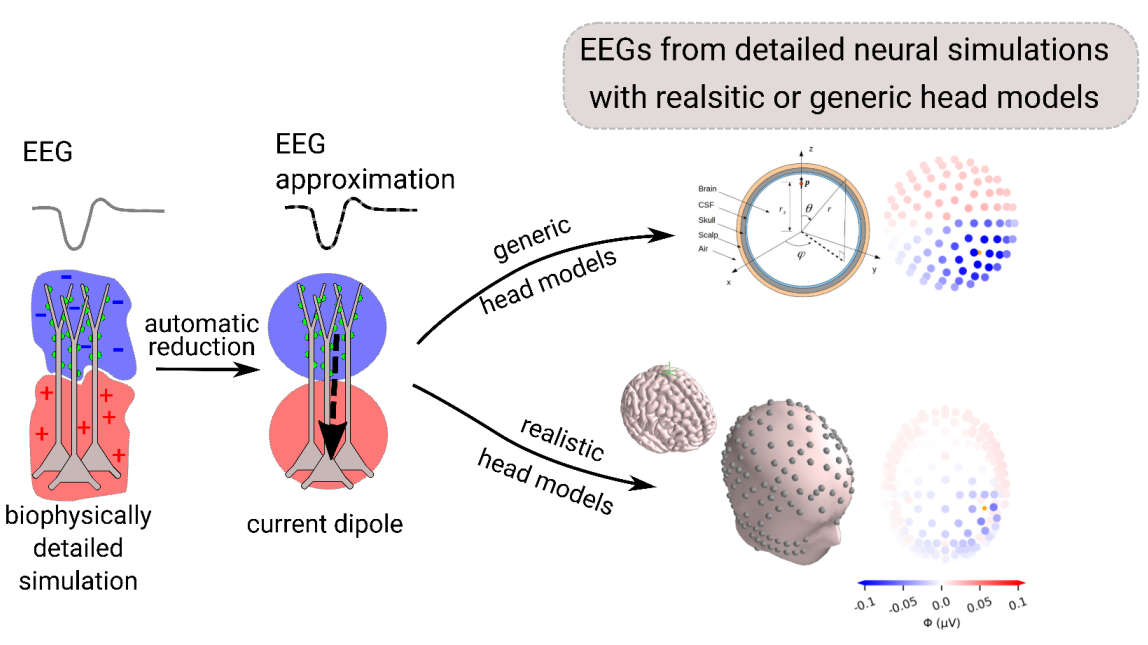
\includegraphics[width=1.0\textwidth]{graph_abst}
	\textbf{Graphical abstract}.
\end{figure}



\section*{Higlights}
\begin{itemize}
\item Current dipoles are computed from biophysically detailed simulated neuron and network activity
\item Extracted current dipoles used in computation of EEG and MEG signals in simplified and detailed head models
\item Method is not suitable for calculating ECoG signals \tvnnote{passer det som Highlight?}
\item Method provides biophysics-based link between detailed neural activity and systems-level signals
\end{itemize}


\section{Introduction}\label{sec:introduction}

Electroencephalography (EEG) is one of the most important non-invasive methods for studying human cognitive function and diagnosing brain diseases \citep{COHEN2017, Pesaran2018}.  Yet, we know surprisingly little about the neural origin of these electric scalp potentials \citep{COHEN2017}: On the one hand, we have a relatively good understanding of the biophysics of EEGs, \tvntxt{in \sntxt{knowing} that these signals originate from cortical current dipoles, and \sntxt{having \sout{ we have}} a well-defined framework for linking such cortical dipoles to electric scalp potentials} \citep{NUNEZ2006}. \sntxt{This has been taken advantage of for a long time in source localization, by inverse modeling of the underlying cortical current dipoles from EEG data. On the other hand, even though these cortical dipoles are assumed to mainly originate from }
large numbers of synaptic input to cortical pyramidal cell populations \citep{NUNEZ2006, SILVA2013, Pesaran2018, Ilmoniemi2019},
\sntxt{the precise link between cortical dipoles and the underlying neural activity has remained unclear. In other words, w}e know very little about exactly which types of neural activity that cause even the most well-studied characteristics of the EEG signal, such as different types of oscillations (e.g., alpha, beta, and gamma waves) and stereotyped EEG-shapes in response to sensory stimuli (event-related potentials, ERPs) \citep{COHEN2017}. Importantly, these different EEG characteristics are affected in predictable ways by various brain conditions, such as sleep and attention \citep{Klimesch1998, Palva2011, Siegel2012}, and by brain disorders including epilepsy and schizophrenia \citep{Niedermeyer2003, Light2013, Freestone2015, MAKI2019}. 
This means that a better insight into how different types of brain activity is reflected in \tvntxt{\sout{EEG signals} cortical current dipoles} could help us in \tvntxt{making better inverse models, } understanding the human brain and curing brain diseases  \citep{Uhlirova2016, COHEN2017, MAKI2019}.
\gen{I also think the possibility for making better inverse models could be mentioned as a motivation.}
\snnote{Har prøvd å bake dette inn nå, litt implisitt kanskje?}
\tvnnote{Hva med dette?}
\snnote{Ja, mye bedre!=)}

The reason why we lack understanding of the neural origin of EEG signals is multifaceted. Among the main causes are (i) strong ethical constraints on invasive human brain measurements and (ii) the high number of neurons that contribute to the signal. However, in recent years there have been major advances in several relevant branches of neuroscience, meaning that a better understanding of the EEG signal may now be within reach \citep{Uhlirova2016, COHEN2017}.

To bypass challenge (i), we look to the rapid development in the technology and methods used to study neural activity in lab animals. The possibility to control and manipulate neural activity, while simultaneously recording both intracranial signals like the local field potential (LFP) \citep{Einevoll2007, Blomquist2009} and extracranial non-invasive signals like the EEG \citep{BRUYNS2017}, can be expected to make important contributions to our understanding of non-invasive measurements of human brain activity \citep{SILVA2013, Uhlirova2016, COHEN2017, Pesaran2018}. 
Furthermore, detailed biophysical modeling of neural activity has become an important tool for understanding intracranial LFP measurements \citep{EINEVOLL2013REVIEW, Pesaran2018}. Given that EEG is expected to reflect the same basic process as LFP, that is, large numbers of synaptic input to geometrically aligned pyramidal cells \citep{NUNEZ2006, Pesaran2018, BUZSAKI2012}, 
%\gen{I suggest we here also add a reference to the review paper in Nature Reviews Neuroscience of Buzsaki et al in 2012.} 
it seems likely that detailed biophysical modeling can also help shed light on the neural origin of EEG signals.

As indicated in challenge (ii), EEG signals are expected to reflect the activity of much larger neural populations than the LFPs, making the simulations computationally demanding. Biophysically detailed large-scale simulations of neural networks have, however, been gaining substantial momentum in recent years, thanks to large ongoing neuroscience initiatives like Project MindScope at the Allen Institute for Brain Science, the Blue Brain Project
and the EU Human Brain Project \citep{EINEVOLL2019}. The possibility to calculate EEG signals from such existing and future large-scale biophysically detailed neural simulations could lead to valuable insights into the neural origin of the EEG.

Another complicating aspect of EEG modeling, is that these predictions in general require a head model to account for the widely different electrical conductivities of the brain, cerebrospinal fluid (CSF), skull and scalp \citep{NUNEZ2006, Ilmoniemi2019}. While many such head models exist, they tend to take current dipoles as input \citep{NUNEZ2006, Pesaran2018}, instead of the transmembrane currents that are available from biophysical neural simulations and that form the basis for modeling LFPs \citep{EINEVOLL2013BOOKCHAPTER}. 

Here, we introduce an approach for reducing arbitrary biophysically detailed simulated neural activity to current dipoles, \sntxt{which represents an enormous reduction of complexity. We verify that the approach is useful} for calculating EEG signals\sntxt{, but less so for ECoG signals. Next, we look into} how the approach can be applied for investigating the origin of EEG signals, \tvntxt{with a particular focus on calcium spikes,} before demonstrating how our methods can be applied for pre-existing large-scale network models. Finally, we show how current dipoles can be combined with \tvntxt{detailed} head models, which enables simulation of EEG signals with unprecedented biophysical detail.  

%\sntxt{Modeling of measurable brain signals applying two separated steps, that is i) current dipole modeling from neural simulations and ii) using a head model to predict measurable brain signals from current dipoles, is common for both EEG and MEG predictions \citep{Ilmoniemi2019}. The general methods presented here can, therefore, analogously be applied for MEG signals.}


\tvntxt{Note that the clear separation between calculation of current dipoles and the corresponding EEG is equally valid for magnetoencephalography (MEG) signals. While we here focus mostly on EEG, the presented approach for calculating current dipoles from neural activity is equally valid for MEG signals, through using an appropriate forward model \citep{Ilmoniemi2019}.}

%\gen{We should also mention ECoG and MEG}


%%%%%%%%%%%%%%%%%%%%%%%%%%%%%%%%%%%%%%%%%%%%%%%%%%%%%%%%%%%%%%%%%%%%%%%%
%%%%%%%%%%%%%%%%%%%%%%%%%%%%%%%METHODS%%%%%%%%%%%%%%%%%%%%%%%%%%%%%%%%%%
%%%%%%%%%%%%%%%%%%%%%%%%%%%%%%%%%%%%%%%%%%%%%%%%%%%%%%%%%%%%%%%%%%%%%%%%
\section{Methods}\label{sec:methods}
Neural activity generates electric currents in the brain, which in turn create electromagnetic fields. In this section, we explain how electric brain signals can be modeled in both simple and more complex volume conductors.

\subsection{Forward modeling of electric potentials}
Due to negligibility of capacitive effects in the head, electric and magnetic signals effectively decouple, and we can apply the quasistatic approximation of Maxwell's equations for calculating these signals \citep{HAMALAINEN1993,NUNEZ2006}. In other words, for computing extracellular electric potentials, we envision the head as a 3D volume conductor, and combining Maxwell's equations with the current conservation law, we obtain the Poisson equation for computing extracellular potentials \cite{GRIFFITHS1999}:
%%%
\begin{equation} \label{eq:poisson}
\mathbf{\nabla} \cdot \mathbf{J} = \mathbf{\nabla}  \cdot (\sigma \mathbf{\nabla} \phi)~,
\end{equation}
where $\mathbf{J}$ is the current density in extracellular space, $\sigma$ is the extracellular conductivity and $\phi$ is the extracellular, electric potential.
%\gen{Her maa vi spesifisere hva som menes med primary current density i vaar kontekst.}
The Poisson equation can be solved analytically for simple, symmetric head models, such as an infinitely big space and spherically symmetric models. For more complex head models, numerical methods such as the Finite Element Method (FEM) can be applied.

\subsubsection{Compartment-based approach}\label{subsubsec:multicomp}
Extracellular potentials generated by transmembrane currents can be calculated with a well-founded biophysical two-step forward-modeling scheme. The first step involves \textit{multicompartmental modeling} and incorporates the details of reconstructed neuron morphologies for calculating transmembrane currents \citep{STERRATT2011}. In the second step, Equation~\eqref{eq:poisson} is solved under the assumption that the extracellular medium is an infinitely large, linear, ohmic, isotropic, homogeneous and frequency-independent volume conductor. The transmembrane currents entering and escaping the extracellular medium can be seen as current sources and sinks, and give the extracellular potential $\phi$ at the electrode location $\mathbf{r}$,
\begin{equation}
\phi(\mathbf{r}) = \frac{1}{4 \pi \sigma}\sum_{n=1}^N \frac{I_n}{|\mathbf{r} - \mathbf{r}_n|}~,
\label{eq:point_source}
\end{equation}
where $\mathbf{r}_n$ is the location of transmembrane current $I_n$, $N$ is the number of transmembrane currents and $\sigma$ is the extracellular conductivity. 
This scheme is here referred to as the compartment-based approach, and was applied using the Python package \texttt{LFPy 2.0} running NEURON under the hood \citep{HAGEN2018,CARNEVALE2006}.

\subsubsection{Current dipole approximation}\label{subsec:cda}
Analogous to how electric charges can create charge multipoles, a combination of current sinks and ources can set up \textit{current} multipoles \citep{NUNEZ2006}. From electrodynamics, we know that extracellular potentials from a volume of current sinks and sources can be precisely described by expressing Equation~\ref{eq:point_source} as a multipole expansion \citep{NUNEZ2006}:
\begin{equation}\label{eq:multipole_expansion}
\phi(R) = \frac{C_{\text{monopole}}}{R} + \frac{C_{\text{dipole}}}{R^2} + \frac{C_{\text{quadrupole}}}{R^3} + ...~,
\end{equation}
when the distance R from the center of the volume to the measurement point is larger than the distance from the volume center to the most peripheral source \citep{JACKSON1998}.
%For definitions of the monopole contribution $C_{\text{monopole}}$, dipole contribution $C_{\text{dipole}}$, quadrupole contribution $C_{\text{quadrupole}}$, see \cite{RIERA2012}.
%\tvnnote{Usikker på om vi bør bruke denne referansen, da litt av poenget i den artikkelen er at de ser monopoler? Har vi en annen? Se Gratiy, Pettersen, Einevoll, Dale (2013) Pitfalls in the interpretation of multielectrode data: on the infeasibility of the neuronal current-source monopoles. J Neurophysiol 109:1681–1682.} 
%\snnote{Aha!! Dette hadde jeg ikke fått med meg! Helt enig! Jeg klarer ikke å finne noen kilde som oppgir disse leddene for strømkilder (ikke ladninger). Går vel kanskje greit å ikke sitere noen her?} \tvnnote{Ja, kanskje bare evt legge inn sitering til bok-kapittelet vårt senere :-)}
%\snnote{smart!}
In neural tissue, the current monopole contribution is zero due to current conservation, since the transmembrane currents sum to zero at all times \citep{Koch1999, PETTERSEN2012}. Further, the quadrupole, octopole and higher order terms are negligible compared to the current dipole contribution when $R$ is sufficiently large.  Therefore, the extracellular potential from a neuron simulation can be estimated with the second term of the current multipole expansion; an approximation known as the \textit{current dipole approximation} \citep{PETTERSEN&EINEVOLL2008,PETTERSEN2014,NUNEZ2006}:
%%%
\begin{equation}\label{eq:dipole_approx}
\phi(\mathbf{r}) = \frac{C_{\text{dipole}}}{R^2} =\frac{1}{4 \pi \sigma} \frac{|\mathbf{p}| \cos \theta}{|{\bf r} - {\bf r}_\mathrm{p}|^2}~.
\end{equation}
%%%
Here, $\mathbf{p}$ is the current dipole moment in a medium with conductivity $\sigma$, $R = |{\bf R}| = |{\bf r} - {\bf r}_\mathrm{p}|$ is the distance between the current dipole moment at ${\bf r}_\mathrm{p}$ and the electrode location ${\bf r}$, and $\theta$ denotes the angle between $\mathbf{p}$ and $\mathbf{R}$.
The current dipole moment ${\bf p}$ can be calculated from an axial current $I$ inside a neuron and the distance vector ${\bf d}$ traveled by the axial current: ${\bf p} = I{\bf d}$, analogous to a charge dipole moment. 
The current dipole approximation is applicable in the far-field limit, that is when $R$ is much larger than the dipole length 
$d = |{\bf d}|$ \citep{NUNEZ2006}. 
%\gen{Synes ikke disse omtrentlige maalene for "applicable" (for what?) er nodvendige.}

%\snnote{I think I've been a bit back and forth regarding how exact the multi-dipole strategy is. Here's a summary after my final derivations: When inserting dipoles generated from a single current sink and a single current source into eq.4, you get no quadrupole,hexadecapol contribution, etc.. But there will be an octopole contribution (and a  $1/R^6$-contribtuion, $1/R^8$-contribution, etc). The multi-dipole approach is therefore not mathematically equivalent to the compartment-based approach (it is based on the current-dipole aproximation, after all). However, since the dipoles are tiny, the distance from the cell giving a neglibible octopole term is much closer here than for the big dipole length in the single-dipole approximation. I'm still not sure whether it would be better to call it the multi-dipole \textit{approach} or \textit{approximation}, since this is an approximation after all...}

\paragraph{Multi-dipole approach}\label{par:multi_dip}

From some multicompartmental neuron simulations (Figure \ref{fig:dipole_field}- \ref{fig:eeg_compare_cell_types}), we computed multiple current dipole moments, i.e., one for each axial current flowing between neighboring compartments in the neuron:
\begin{equation}
{\bf p}_k = I_k^{\mathrm{axial}} {\bf d}_k.
\end{equation}
Here, $I_k^{\mathrm{axial}}$ is an axial current traveling along distance vector ${\bf d}_k$, resulting in a current dipole moment ${\bf p}_k$.
%\tvntxt{\sout{Each of these current dipole moments contributes to the extracellular potential. }}
By inserting all the current dipole moments from a neuron simulation into the current dipole approximation (Equation~\ref{eq:dipole_approx}), we get a good estimate of the extracellular potential at any electrode location where the distance between the electrode and the nearest dipole is sufficiently large 
%\sout{shorter than three or four times this dipole's length}
\citep{NUNEZ2006}.
Note that the length of each (multi-)dipole is equal to half the length of its corresponding neuronal compartment. %This means that each dipole is quite short (normally on the scale of a few tens of micrometers), meaning that the multi-dipole approach is normally a very good approximation at distances larger than 50-100 $\si{\mu m}$ from the neuron. \tvnnote{Tenker egentlig vi kan droppe siste setning} \snnote{Ja!}


%Note that these (multi-)dipoles are quite short (normally on the scale of a few tens of micrometers), meaning that the multi-dipole approach is normally a very good approximation at distances larger than 50-100 $\si{\mu m}$ from the neuron.
%\snnote{Maybe exclude the last sentence above? I only checked the segev 3a cell, and the largest dipole length was 12.5 micrometers, that's all it's based on.}
%\tvnnote{Jeg syntes den er lur å ha med, men kanskje koble det tydligere opp mot lengden på compartments i morfologiene?}
%\snnote{Noe sånt?}

\paragraph{Single-dipole approximation}\label{par:single_dip}
From each multicompartmental neuron simulation, we computed one single current dipole moment. This can either be done by summing up the multiple current dipole moments,

\begin{equation}\label{eq:dip_sum_axial}
\mathbf{p}(t) = \sum_{k=1}^{M} {\bf p}_k(t) = \sum_{i=1}^{M} I_k^{\mathrm{axial}}(t) \mathbf{d}_k,
\end{equation}
where $M$ is the number of axial currents,
or equivalently from a position-weighted sum of all the transmembrane currents \citep{LINDEN2010, HAGEN2018}:

\begin{equation}\label{eq:dip_sum_trans}
\mathbf{p}(t) = \sum_{k=1}^{N} I_k^{\mathrm{trans}}(t) \mathbf{r}_k,
\end{equation}
where N is the number of compartments in the multicompartmental neuron model and ${\bf r}_k$ is the position of transmembrane 
current $I_k^{\mathrm{trans}}(t)$.
The calculation of current-dipole moments from simulated neural activity was implemented in LFPy 2.0, and can used through \texttt{Cell.current\_dipole\_moment}  \citep{HAGEN2018}.


%Combining the single current dipole moment with the current dipole approximation gives us the extracellular potential from a single neuron in the far-field limit ($R>3d$ or $4d$) \citep{NUNEZ2006}. \tvnnote{Trengs kanskje ikke?}


% Each of these current dipole moments will contribute to the extracellular potential from a neuron. And when assuming that our measurement points are further away from the dipole than the dipole length itself, we can plug the current dipole moments into the multipole expansion, and since the dipole contribution will be the only term contributing from a pure current dipole moment, the axtracellular potential 
%
%\begin{equation}
%\phi^{multi}_k(\mathbf{r}) =\frac{1}{4 \pi \sigma} \frac{|{\bf p}_k| \cos \theta}{|{\bf r} - {\bf r}_k |^2}~,
%\label{eq:dipole}
%\end{equation}
%
%where ${\bf r}_k$ is the location of current dipole moment ${\bf p}_k$. 
%



%The simplest possible neuron model from which we can calculate the current dipole moment is a  two-compartmental neural stick, where one compartment will act as a current sink and the other as a current source. The current dipole moment from this model, can be defined as the axial current from the current sink to the current source, times the distance between the sink and the source:
%
%\begin{eqnarray}
%{\bf p} = I^{axial}{\bf d}.
%\end{eqnarray}
%For this two-compartment model, $I^{axial} = I_{source} = I_{sink}$ and ${\bf d} = {\bf r}_{sink} - {\bf r}_{source}$
% Applying the point-source approximation and Kirchhoff's current law, we obtain the following relation:
%\begin{equation}\label{eq:dip_trans_to_axial}
%\mathbf{p} = I_{source} \mathbf{r}_{source} + I_{sink} \mathbf{r}_{sink}
%= I \mathbf{r}_{source} - I \mathbf{r}_{sink}
%= I (\mathbf{r}_{source} - \mathbf{r}_{sink}) = I \mathbf{d}~,
%\end{equation}
%where $\mathbf{d}$ denotes the distance between the two compartments, and $I$ is the axial current. Generalizing this relation to an N-compartment neuron model, we can calculate the current dipole moment by summing up multiple current dipole moments $\mathbf{p}_i^{multi}$, computed from axial currents $I_i^{axial}$ between neighboring compartments $i$ and $i+1$, separated by a distance $\mathbf{d}_i$:
%\begin{equation}\label{eq:dip_sum_axial}
%\mathbf{p}(t) = \sum_{i=1}^{N-1} I_i^{axial}(t) \mathbf{d}_i
%= \sum_{i=1}^{N-1} \mathbf{p}_i^{multi}(t)  ~.
%\end{equation}
%
%
%
%
%
%The current dipole moment can be calculated from transmembrane currents as follows:
%\begin{equation}\label{eq:dip_sum_trans}
%\mathbf{p}(t) = \sum_{n = 1}^{N} \mathbf{r}_n I_n(t)~,
%\end{equation}
%where $I_n$ is the transmembrane current in compartment $n$ at position $\mathbf{r}_n$.
%
%
%
%%Equations~\eqref{eq:dip_sum_trans}-\eqref{eq:dip_sum_axial} apply the point-source approximation. For proof of equality between the point-source and the line-source approximation when computing the current dipole moment from neuron simulation, see~\ref{sec:point_line_cdm}.


\subsection{Head models}
Electric potentials will be affected by the geometries and conductivities of the various parts of the head \citep{NUNEZ2006}, which is especially important for electrode locations outside of the brain. This can be incorporated into our extracellular potential calculations by applying simplified or complex head models.

\subsubsection{Four-sphere model}\label{subsubsec:4S}
The four-sphere head model is a simple analytical model consisting of four concentric shells: brain tissue, cerebrospinal (CSF) fluid, skull and scalp, where the conductivity can be set individually for each shell \citep{SRINIVASAN1998,NUNEZ2006}\sntxt{, see Table~\ref{tab:4sphere} for parameters used in this paper.} The model solution is given in \cite{NAESS2017} and is found by solving the Poisson equation subject to boundary conditions ensuring continuity of current and electric potentials over the boundaries, as well as no current escaping the outer shell. This model is based on the current dipole approximation.


\begin{table*}[ht]
  \centering
  \begin{tabular}{c|c|c}
    \hline
    \rule{0pt}{2ex}  & Radius (\si{cm}) & $\sigma$ (\si{S/m}) \\ 
    \hline 
    \rule{0pt}{2ex} Brain & 7.9 & 0.3 \\ 
    CSF & 8.0 & 1.5 \\ 
    Skull & 8.5 & 0.015 \\ 
    Scalp & 9.0 & 0.3 \\ 
    \hline
  \end{tabular}
  \caption{\sntxt{\textbf{Radii and electrical conductivities used in the four-sphere model.} The radius of each spherical shell in the four-sphere model is given in centimeters, while $\sigma$ denotes the respective electrical conductivity in the unit of \si{S/m}.}}
  \label{tab:4sphere}
\end{table*}

\subsubsection{New York Head model}\label{subsubsec:NYH}
The New York Head model is a detailed head model based on high-resolution, anatomical MRI-data from 152 adult heads \citep{HUANG2015}. The model was constructed by taking advantage of the reciprocity theorem, stating that the position of the electrode and the dipolar source can be switched without affecting the measured potential \citep{RUSH1969}. This means, that virtually injecting current at the locations of the EEG electrodes and using the finite element method \citep{LOGG2012} to compute the resulting potential anywhere in the brain, gives the link between current dipoles in the brain and the resulting EEG signals \citep{Malmivuo1995, Ziegler2014, HUANG2016, Dmochowski2017}.
%\gen{Ja, det er kanskje saa enkelt?} 
This link was captured in a matrix known as the \textit{lead field} ${\bf L}$ \citep{NUNEZ2006}: 

\begin{equation}
{\bf L} = \frac{{\bf E}}{I}
\end{equation}
Here, $I$ is the injected current at the electrode locations and ${\bf E}$ is the resulting electric field in the brain. The lead field matrix gives us the precise link between a current dipole moment ${\bf p}$ in the brain and the resulting EEG signals ${\bf \Phi}$ \citep{NUNEZ2006}:
\begin{equation}
{\bf \Phi} = {\bf L} \cdot {\bf p}.
\end{equation}

We applied the New York Head model by downloading the lead field ${\bf L}$ from \url{parralab.org/nyhead/}. The units incorporated in the lead field matrix was not immediately obvious. However, from \cite{Dmochowski2017,HUANG2013} it appears that an injected current $I$ of 1 mA gives an electric potential $E$ in V/m, meaning that the lead field brings us from a current dipole moment ${\bf p}$ in the unit of mAm to EEG signals in the unit of V.


%The New York head model is an example of a numerical, complex head model based on 152 adult heads. In the New York Head Model, the link between current dipoles in the brain and resulting EEG signals was established using the finite element method \citep{LOGG2012,HUANG2015}. Even though developing such a model comes at a high financial and computational cost, applying the pre-solved model is quite straightforward: inserting a current dipole moment into an arbitrary brain location gives the resulting EEG signals less than a second.\tvnnote{Minutes? Ville trodd mye mindre. Nevne reciprocity?}\snnote{Obs! Denne hadde jeg glemt å fikse. 0.29s! } \snnote{Synes dette avsnittet er litt kjipt.. Enig i at reciprocity burde være med her. Burde vi isåfall fjerne det fra 3.5? Dette med hvor lang tid det tar å kjøre NYH har vi skrevet mer detaljert under 3.5.. Kunne evt. ha lagt første avsnitt fra 3.5 her og laget en kortere versjon til 3.5?}


\subsection{Simulation of neural activity}\label{subsec:simulation}
All neuron simulations were performed using the python package \texttt{LFPy}, running NEURON under the hood \citep{HAGEN2018}. 
For investigations of single-cell contributions to extracellular potentials, we applied three different morphologically reconstructed cell models: The human layer-23 pyramidal cell from \cite{EYAL2018}, the layer-5 pyramidal cell from rat cortex constructed by \cite{HAY2011} and a rat layer-5 chandelier cell; an interneuron model developed by \cite{MARKRAM2015}.

The pyramidal cell models were downloaded from \url{senselab.med.yale.edu/modeldb/}, with accession numbers 238347 (2013\_03\_06\_cell03\_789\_H41\_03) and 139653 (cell1) respectively, while we found the interneuron at the Neocortical Microcircuit Collaboration Portal (\url{bbp.epfl.ch/nmc-portal/microcircuit}) under layer-5, Chandelier Cell (ChC), continuous Non-accomodating (cNAC), (rp110201\_L\_idA\_-\_Scale\_x1.000\_y0.975\_z1.000\_-\_Clone\_3). %\snnote{There are several morphologies under each of the accession numbers. should we specify exactly which morphology we've used?}
%\tvnnote{Ja, gi navnet på morfologien}

For all simulations with passive ion channels only (Fig.~\ref{fig:dipole_field}-\ref{fig:eeg_compare_cell_types}), 
we used the following cell parameters: membrane resistance of 30000~$\Omega \text{cm}^2$, axial resistance of 150~$\Omega \text{cm}$ \citep{MAINEN1996} and a membrane capacitance of 1~$\mu\text{F}/\text{cm}^2$ %\tvntxt{\sout{(rounded up from}}
\citep{GENTET2000,STERRATT2011}. When active mechanisms were included in the simulations (Fig.~\ref{fig:ca_spike}), all cell properties were incorporated as described in the specific cell's documentation.

Neural simulations shown in Fig.~\ref{fig:dipole_field}-\ref{fig:ca_spike} received synaptic input modeled as conductance-based, two-exponential synapses (\texttt{Exp2Syn} in \texttt{NEURON}). The rise time constant was set to 1 ms and the decay time constant was 3 ms, synaptic reversal potential was 0 mV and the synaptic weight was set to 0.002~\si{\mu S}, unless otherwise specified. %\tvnnote{Gjelder ikke hybrid modellen. Kanskje gi figurnummer?}

%\snnote{Burde denne vaert mer omfattende?:}
%\tvnnote{La på bittelitt, tenker det holder}
For modeling of population activity (Figure~\ref{fig:population},~\ref{fig:compare_head_models}), we  used the so-called hybrid scheme, and the simulation was unmodified from \cite{HAGEN2016}, except that all single-cell current dipole moments were recorded, and the EEG signals calculated.

\subsection{Code availability}
Simulation code to reproduce all figures in this paper is freely available from \url{https://github.com/solveignaess/EEG.git}

%%%%%%%%%%%%%%%%%%%%%%%%%%%%%%%%%%%%%%%%%%%%%%%%%%%%%%%%%%%%%%%%%%%%%%%%
%%%%%%%%%%%%%%%%%%%%%%%%%%%%%%%RESULTS%%%%%%%%%%%%%%%%%%%%%%%%%%%%%%%%%%
%%%%%%%%%%%%%%%%%%%%%%%%%%%%%%%%%%%%%%%%%%%%%%%%%%%%%%%%%%%%%%%%%%%%%%%%
\section{Results}\label{sec:results}
\normalsize

We introduce an approach for modeling \tvntxt{electrocorticography (ECoG), electroencephalography (EEG), and magnetoencephalography (MEG) \sout{electroencephalography (EEG)}} signals from detailed biophysical multicompartment cell models. For illustration, we first consider single synaptic input to single neurons in an infinite homogeneous head model, before moving on to a simple, generic head model. Finally, we study EEGs from \tvntxt{large-scale simulated network} activity, also applying a realistic head model. 
%Note that while we will only consider EEG signals, the general approach is equally valid for MEG signals. 
%\gen{ECoG modelleringen boer vel ogsaa nevnes her.}


%We introduce an approach for detailed biophysical modeling of ECoG, EEG and MEG signals by considering a single synaptic input to a biophysically detailed cell model. 
%
%Note that we will for the most part only consider EEG signals, but the general results are equally valid for MEG signals.

\subsection{At sufficiently large distances, extracellular potentials become dipolar}\label{subsec:cb_db_comp_inf}
%Excitatory synaptic input initiates a negative current at the synaptic input site (positive ions going into the cell), and due to current conservation \citep{NUNEZ2006} this negative current is exactly balanced by spatially distributed positive currents along the cellular membrane, as illustrated in Fig.~\ref{fig:dipole_field}\textbf{A} for a single apical excitatory synaptic input to a human cortical layer 2/3 pyramidal cell model \citep{EYAL2016}. In the standard approach to modeling extracellular potentials, here referred to as the {\it compartment-based approach}, the transmembrane currents of each of the cellular compartments correspond to a point current source/sink, but a mathematically equivalent formulation would be to instead consider the axial current of each cellular compartment as a small current dipole, which we will here refer to as the {\it multi-dipole approach} (Fig.~\ref{fig:dipole_field}\textbf{B}). By summing all these dipoles into a single dipole at a specific position, we obtain the {\it single-dipole approximation} (Fig.~\ref{fig:dipole_field}\textbf{C}).
%
%For illustration we first assume that the cell is positioned in an infinite homogeneous medium, in which case the extracellular potential can be easily calculated by the compartment-based approach (eq.~\ref{eq:point_source}) or from the multi-dipole or single-dipole approximation (eq.~\ref{eq:dipole}). Very close to the cell the extracellular potential will strongly depend on the exact distribution of transmembrane currents across the cellular morphology, and it will therefore typically not have the shape of a single dipole (Fig.~\ref{fig:dipole_field} \textbf{D,E} versus \textbf{F}). However, since the extracellular potential
%can be expressed as a multipole expansion (eq.~\ref{eq:dipole_expansion}) and all higher order terms will decay faster with distance than the dipole term, the extracellular potential becomes increasingly dipolar with distance from the cell \citep{LINDEN2010}, meaning that for the purpose of calculating extracellular potentials far away from the cell, the single-dipole approximation might be well justified (Fig.~\ref{fig:dipole_field}\textbf{G-I}).

%\sntxt{
%	
%In this section, we compare three strategies for computing extracellular potentials: the compartment-based approach, the multi-dipole approach and the single-dipole approximation.
%While the first is a well-established method for computing extracellular potentials in homogeneous volume conductors,
%%(in addition to studies such as \cite{NESS2016})
% inhomogeneous head models typically take current dipole moments as input, and must be based on approximations such as the latter two. In order to understand the differences between the three strategies, we here compare single-cell extracellular potentials modeled close to the cell, and the potential in the far-field limit.
%%\linebreak
%%The standard way of modeling extracellular potentials in homogeneous volume conductors is to apply the so-called compartment-based approach \ref{subsubsec:multicomp}. However, 
%\linebreak
%When computing extracellular potentials in neural tissue, well-established compartment-based approach based on transmembrane currents. Dipole-based approaches for modeling of extracellular potentials further away from the neuronal sources are important for two reasons: Firstly, 
%
%When it comes to inverse modeling of extracellular potentials further away from the neuronal sources, on the other hand, such as EEG and MEG, the goal is to find the neuronal sources in the form of current dipole moments; not transmembrane currents. In this section, we 
%
%(Section~\ref{subsubsec:multicomp}) in an infinite homogeneous medium is well jstified. When it comes to modeling electromegnetic signals further away from neuronal sources, like EEG and MEG, 
%
%Here, we investigate the extracellular potential of a single neuron in order to compare to dipole-based approaches with the 
%
%
%The standard forward-modeling scheme for extracellular potentials model extracellular potentials from neurons' transmembrane currents. When it comes to inverse modeling of EEG/MEG, on the other hand, the goal is to find the current dipole moments from the measured electromagnetic signals. Also, applying 
%}

%\tvnnote{Can we find a simple one-sentence motivation for why we might want to do this? Maybe start paragraph by breifly introducing why we want to go from compartment-based to dipole-based?}
%\snnote{Tuesday, we discussed that the overall motivation for going from compartment-based to dipole-based is 1) we need dipoles for head models and 2) inverse methods model dipoles, not currents. I wrote a short draft on this paragraph in the Introduction, so that we don't forget to spell this out there. Since the Results section should be able to stand alone, I guess it makes sense to mention this here as well. I found it very hard to make an easy-to-read one-sentence motivation here. Is it ok to skip part 2 of the motivation, in order to make this shorter, and assume that the reader goes through the introduction, if she wants the full story? I came up with a suggestion where I feel like the flow is ok, and that it leads up nicely to the rest of the section, but even though leaving out motivation part 2, I didn't manage to keep it within one sentence. Is this ok, or do you have any other suggestions?=)}

%We start by comparing three strategies for computing extracellular potentials: the compartment-based approach, the multi-dipole approach and the single-dipole approximation.
%While the first is a well-established method for computing extracellular potentials in homogeneous volume conductors,
%(in addition to studies such as \cite{NESS2016})
%inhomogeneous head models typically take current dipole moments as input, and must be based on approximations such as the latter two. In order to understand the differences between the three strategies, we here compare extracellular potentials generated by a single cell receiving excitatory synaptic input.

When modeling electric potentials within the brain, we can apply the well-established compartment-based approach assuming a homogeneous volume conductor (section \ref{subsubsec:multicomp}) \citep{EINEVOLL2013REVIEW,HOLT1999}.
%\gen{Kan vel ogsaa referere til Holt \& Koch her.}
However, this assumption is no longer valid when it comes to modeling EEG signals on the scalp, which calls for an inhomogeneous head model \citep{Ilmoniemi2019}. Such head models typically take current dipoles as input, as opposed to individual current sinks/sources, and must be based on the current dipole approximation \citep{NUNEZ2006}. Here, we introduce an approach for computing current dipoles from arbitrary simulated neural activity, and compare current-based and dipole-based modeling of electric potentials generated by a single cell receiving excitatory synaptic input.
%The neural activity underlying EEG signals is predominantly thought of as transmembrane currents. However, when it comes to inverse modeling of these signals, one estimates the origin of neural activity as current dipoles, instead of currents. Applying head models for computing EEG signals typically take 
Excitatory synaptic input initiates a negative current at the synapse location, since positive ions flow into the cell. Due to current conservation \citep{Koch1999}, this negative current is exactly balanced by spatially distributed positive currents along the cellular membrane, as illustrated in Fig.~\ref{fig:dipole_field}\textbf{A} for a single apical excitatory synaptic input to a passive human cortical layer-2/3 pyramidal cell model \citep{EYAL2016}.See Methods \ref{subsec:simulation} for simulation details.
%\sntxt{The simulation lasted 100 ms, with the synaptic input occurring after 20ms.}
%\tvnnote{Kan fjernes siden det er i figurtekst}
%\snnote{Maybe these terms will be defined in the methods section?}
%\tvnnote{I don't feel we have to introduce them, but maybe cite a basic textbook?}
In the standard procedure for modeling extracellular potentials, here referred to as the {\it compartment-based approach}, the transmembrane current in each cellular compartment corresponds to a point current source/sink. Another strategy is to consider the axial current of each cellular compartment as a small current dipole (see Equation~\eqref{eq:dip_sum_axial}), which we will refer to as the {\it multi-dipole approach} (Fig.~\ref{fig:dipole_field}\textbf{B}). By vector summation of all these dipoles into one single dipole at a specific position, we obtain the {\it single-dipole approximation} (Fig.~\ref{fig:dipole_field}\textbf{C}).
For the sake of comparing these modeling approaches, we have assumed that the cell is positioned in an infinite homogeneous electric medium. Very close to the neuron, the extracellular potential will strongly depend on the exact distribution of transmembrane currents across the cellular morphology and  will, therefore, typically not take a purely dipolar shape (Fig.~\ref{fig:dipole_field} \textbf{D,E} versus \textbf{F}). However, since the dipole contribution will dominate when we are further away from the current sources (see Equation~\ref{eq:multipole_expansion}), the extracellular potential becomes more and more dipolar with increasing distance from the cell \citep{LINDEN2010}. This implies that for the purpose of calculating extracellular potentials far away from the cell, the single-dipole approximation might be well justified (Fig.~\ref{fig:dipole_field}\textbf{G-I}). Note that there can be small differences between the results from the compartment-based and the multi-dipole approaches for electrode locations in the immediate vicinity of the current sources, due to the approximations inherent in using the current dipole model (Fig.~\ref{fig:dipole_field}D versus Fig.~\ref{fig:dipole_field}E).
%immediate vicinity of the neuron
%\tvnnote{Kanskje heller si "immediate vicinity of the current sources, due to the assumptions in the current dipole approximation" eller noe slikt? Tenker også vi kan droppe resten av setningen}
%\snnote{jepp!}
 %, however for the electrode locations considered in the rest of this paper, these differences will be negligible.

%For electrode locations in the immediate vicinity of the neuron, it is possible to see tiny differences between the compartment-based and the multi-dipole approaches, however

%\tvnnote{Here, I have used the terms compartment-based \textbf{approach}, multi-dipole \textbf{approach} and single-dipole \textbf{approximation}, but I'm not sure about that.}

%The applicability of the single-dipole model, as compared to the multicompartmental model, was tested in the simplest volume conductor possible, i.e. an infinite 3D volume conductor with constant conductivity. The extracellular medium conductivity was set to $0.3$~S/m \cite{HAMALAINEN1993,LOGOTHETIS2007,NUNEZ2006} and we used the Segev cell for the neuron simulation, as described in Section \ref{subsec:neuron_models}. A single excitatory synapse was placed on an apical dendrite, generating an exponential synaptic input current. Figure~\ref{fig:dipole_field} illustrates the difference in electric potential modeled with the multicompartmental, multi-dipole and single-dipole models, but also how the models give interchangeable results in the far-field limit.
	
\begin{figure}[H]
	\centering
	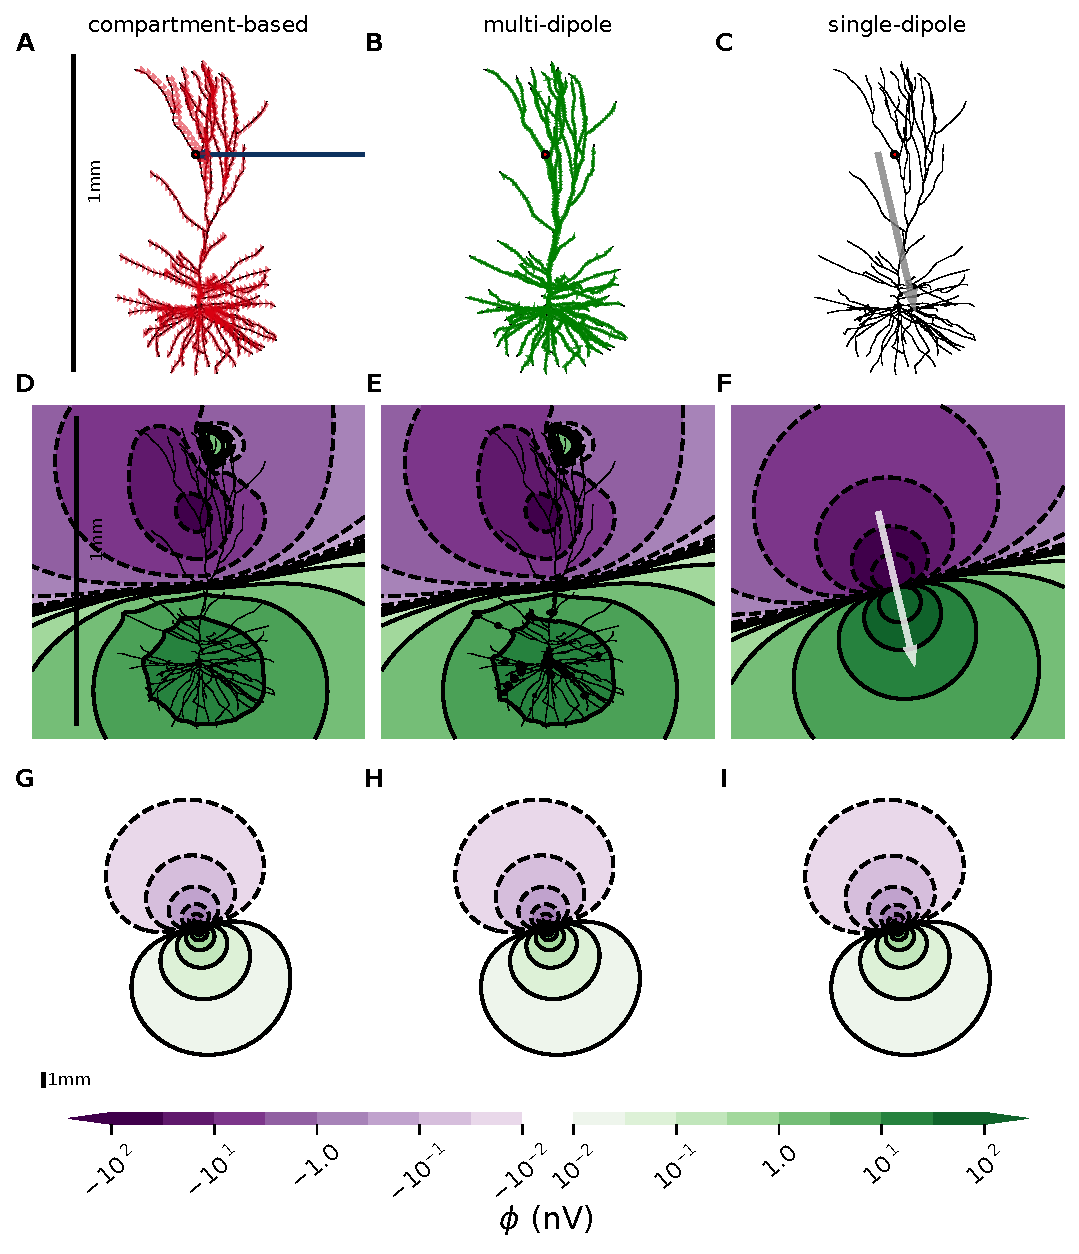
\includegraphics[width=1.0\textwidth]{fig_dipole_field_passiveTrue_single_syn481}
	\caption{\textbf{Extracellular potentials become dipolar in the far field limit}. 
		\textbf{A}: Passive layer 2/3 pyramidal cell from human \citep{EYAL2016} with an excitatory, conductance-based, two-exponential synapse placed on apical dendrite (red dot), see \ref{subsec:simulation}. The resulting transmembrane currents for each compartment are shown as a blue arrow (input current) and red arrows (return currents).
%		\gen{Kanskje bedre aa si at all returstrom er positiv (roed), og at kun synapsestroemmen er negativ (blaa)?}
%		\gen{Maa spesifisere synaptisk str{\o}m. DC?}
		\textbf{B}: Green arrows represent the multiple current dipole moments between neighboring neural compartments.
		\textbf{C}: Gray arrow illustrates the total current dipole moment, that is, the vector sum of the dipoles in B.
	\textbf{D-F}: Extracellular potential in immediate proximity of the neuron, computed with the compartment-based approach, multi-dipole approach and single-dipole approximation, respectively. Note that the multi-dipole results differ slightly from the compartment-based approach when the distance from the measurement point to the nearest current dipole moment is short compared to the dipole length.
\textbf{G-I}: Same as D-F, but at a larger spatial scale (zoomed out). See $1$~mm scalebar in panel A, D and G.
}
\label{fig:dipole_field}
\end{figure}


\subsection{Single-dipole approximation is justified for EEG, but not ECoG signals}\label{subsec:cb_db_comp_4s}

In order to test the applicability of the single-dipole approximation for calculating ECoG and EEG signals, we applied the four-sphere head model \citep{NAESS2017, HAGEN2018, HAGEN2019}.
Since the four-sphere head model takes current dipoles as input, the multi-dipole approach was used as benchmark: an assumption that should be well justified for the cell-to-electrode distances considered, see section \ref{subsec:cb_db_comp_inf}.

For different locations of a single excitatory synaptic input to a human cortical layer-2/3 pyramidal cell model \citep{EYAL2016}
(Fig.~\ref{fig:compare_multi_single_dipole}\textbf{A}), we calculated the electric potential at point-electrode positions spanning from 100 $\mu$m above the top of the cell, to the surface of the head, using both the multi-dipole approach and the single-dipole approximation (Fig.~\ref{fig:compare_multi_single_dipole}\textbf{B}). 
We used conductance-based synapses and included only passive membrane conductances, but we confirmed that instead using current-based synapses or a fully active cell model gave very similar results.  

The electric potential attenuated steeply with distance when crossing the different layers of the head model, most strongly across the low-conducting skull (Fig.~\ref{fig:compare_multi_single_dipole}\textbf{B}). 
For all synaptic input locations, we observed that the electric potential calculated with the single-dipole approximation markedly deviated from the multi-dipole approach directly above the neuron, but the difference strongly decreased with distance from the neuron 
%\gen{Er vel mer vant med at vi bruker ordet "neuron" og ikke "cell" ...}
(Fig.~\ref{fig:compare_multi_single_dipole}\textbf{B}, full versus dashed lines for two selected synapse locations). 
We quantified the model dissimilarities by looking at the relative error, and for a chosen distal synaptic input the relative error was 40.0\% and 1.06\% at the position of the ECoG and EEG electrodes respectively (Fig.~\ref{fig:compare_multi_single_dipole}\textbf{C}, green line). For a specific proximal synaptic input we observed a relative error of 76.1$\%$ at the ECoG position, and 7.61$\%$ at the EEG position (Fig.~\ref{fig:compare_multi_single_dipole}\textbf{C}, purple line). Inserting a single strong synaptic current (synaptic weight 0.05~\si{\mu S}) into the soma of the same layer-2/3 pyramidal cell with active mechanisms \citep{EYAL2018}, resulting in a somatic spike, gave relative errors of 34.7$\%$ and 0.967$\%$ for the computed ECoG and EEG signals, respectively (results not shown).
%\gen{Her maa det spesifiseres litt mer. Hvordan maales signalet? Og hvilken modell er det snakk om? (Ikke lenger bare passive konduktanser som over.)}
%\gen{Kanskje denne oppsummeringssetningen passer best helt til slutt i 3.2? Og "some synaptic locations" er jo litt tamt.}
%\gen{Synes det er vanskelig aa karakterisere en approksimasjon some generelt "justified" - det avhenger jo av hvilke noeyaktighet som trengs i de ulike tilfeller. Synes det er bedre aa si at feilen er mindre enn XX \%.}
We found that calculating EEG signals with the single-dipole approximation gave relative errors peaking for synaptic locations $\sim$ 60 and 400~$\si{\um}$ above the soma (Fig.~\ref{fig:compare_multi_single_dipole}\textbf{D}),
but note that these synaptic input locations also gave relatively weak EEG signals (Fig.~\ref{fig:compare_multi_single_dipole}\textbf{E}).
This demonstrates that the relative error of the single-dipole approximation is negatively correlated with the amplitude of the scalp potential (Fig.~\ref{fig:compare_multi_single_dipole}\textbf{F}).
This is as expected, given that the strongest EEG signals are expected to be caused by dipole-like source/sink distributions (section \ref{subsec:cda}).
\sntxt{In summary, the single-dipole approximation can result in substantial errors at the position of the ECoG electrodes, but give small errors at the position of the EEG electrodes for synaptic locations leading to strong EEG signals.}



\begin{figure}[H]
	\centering
	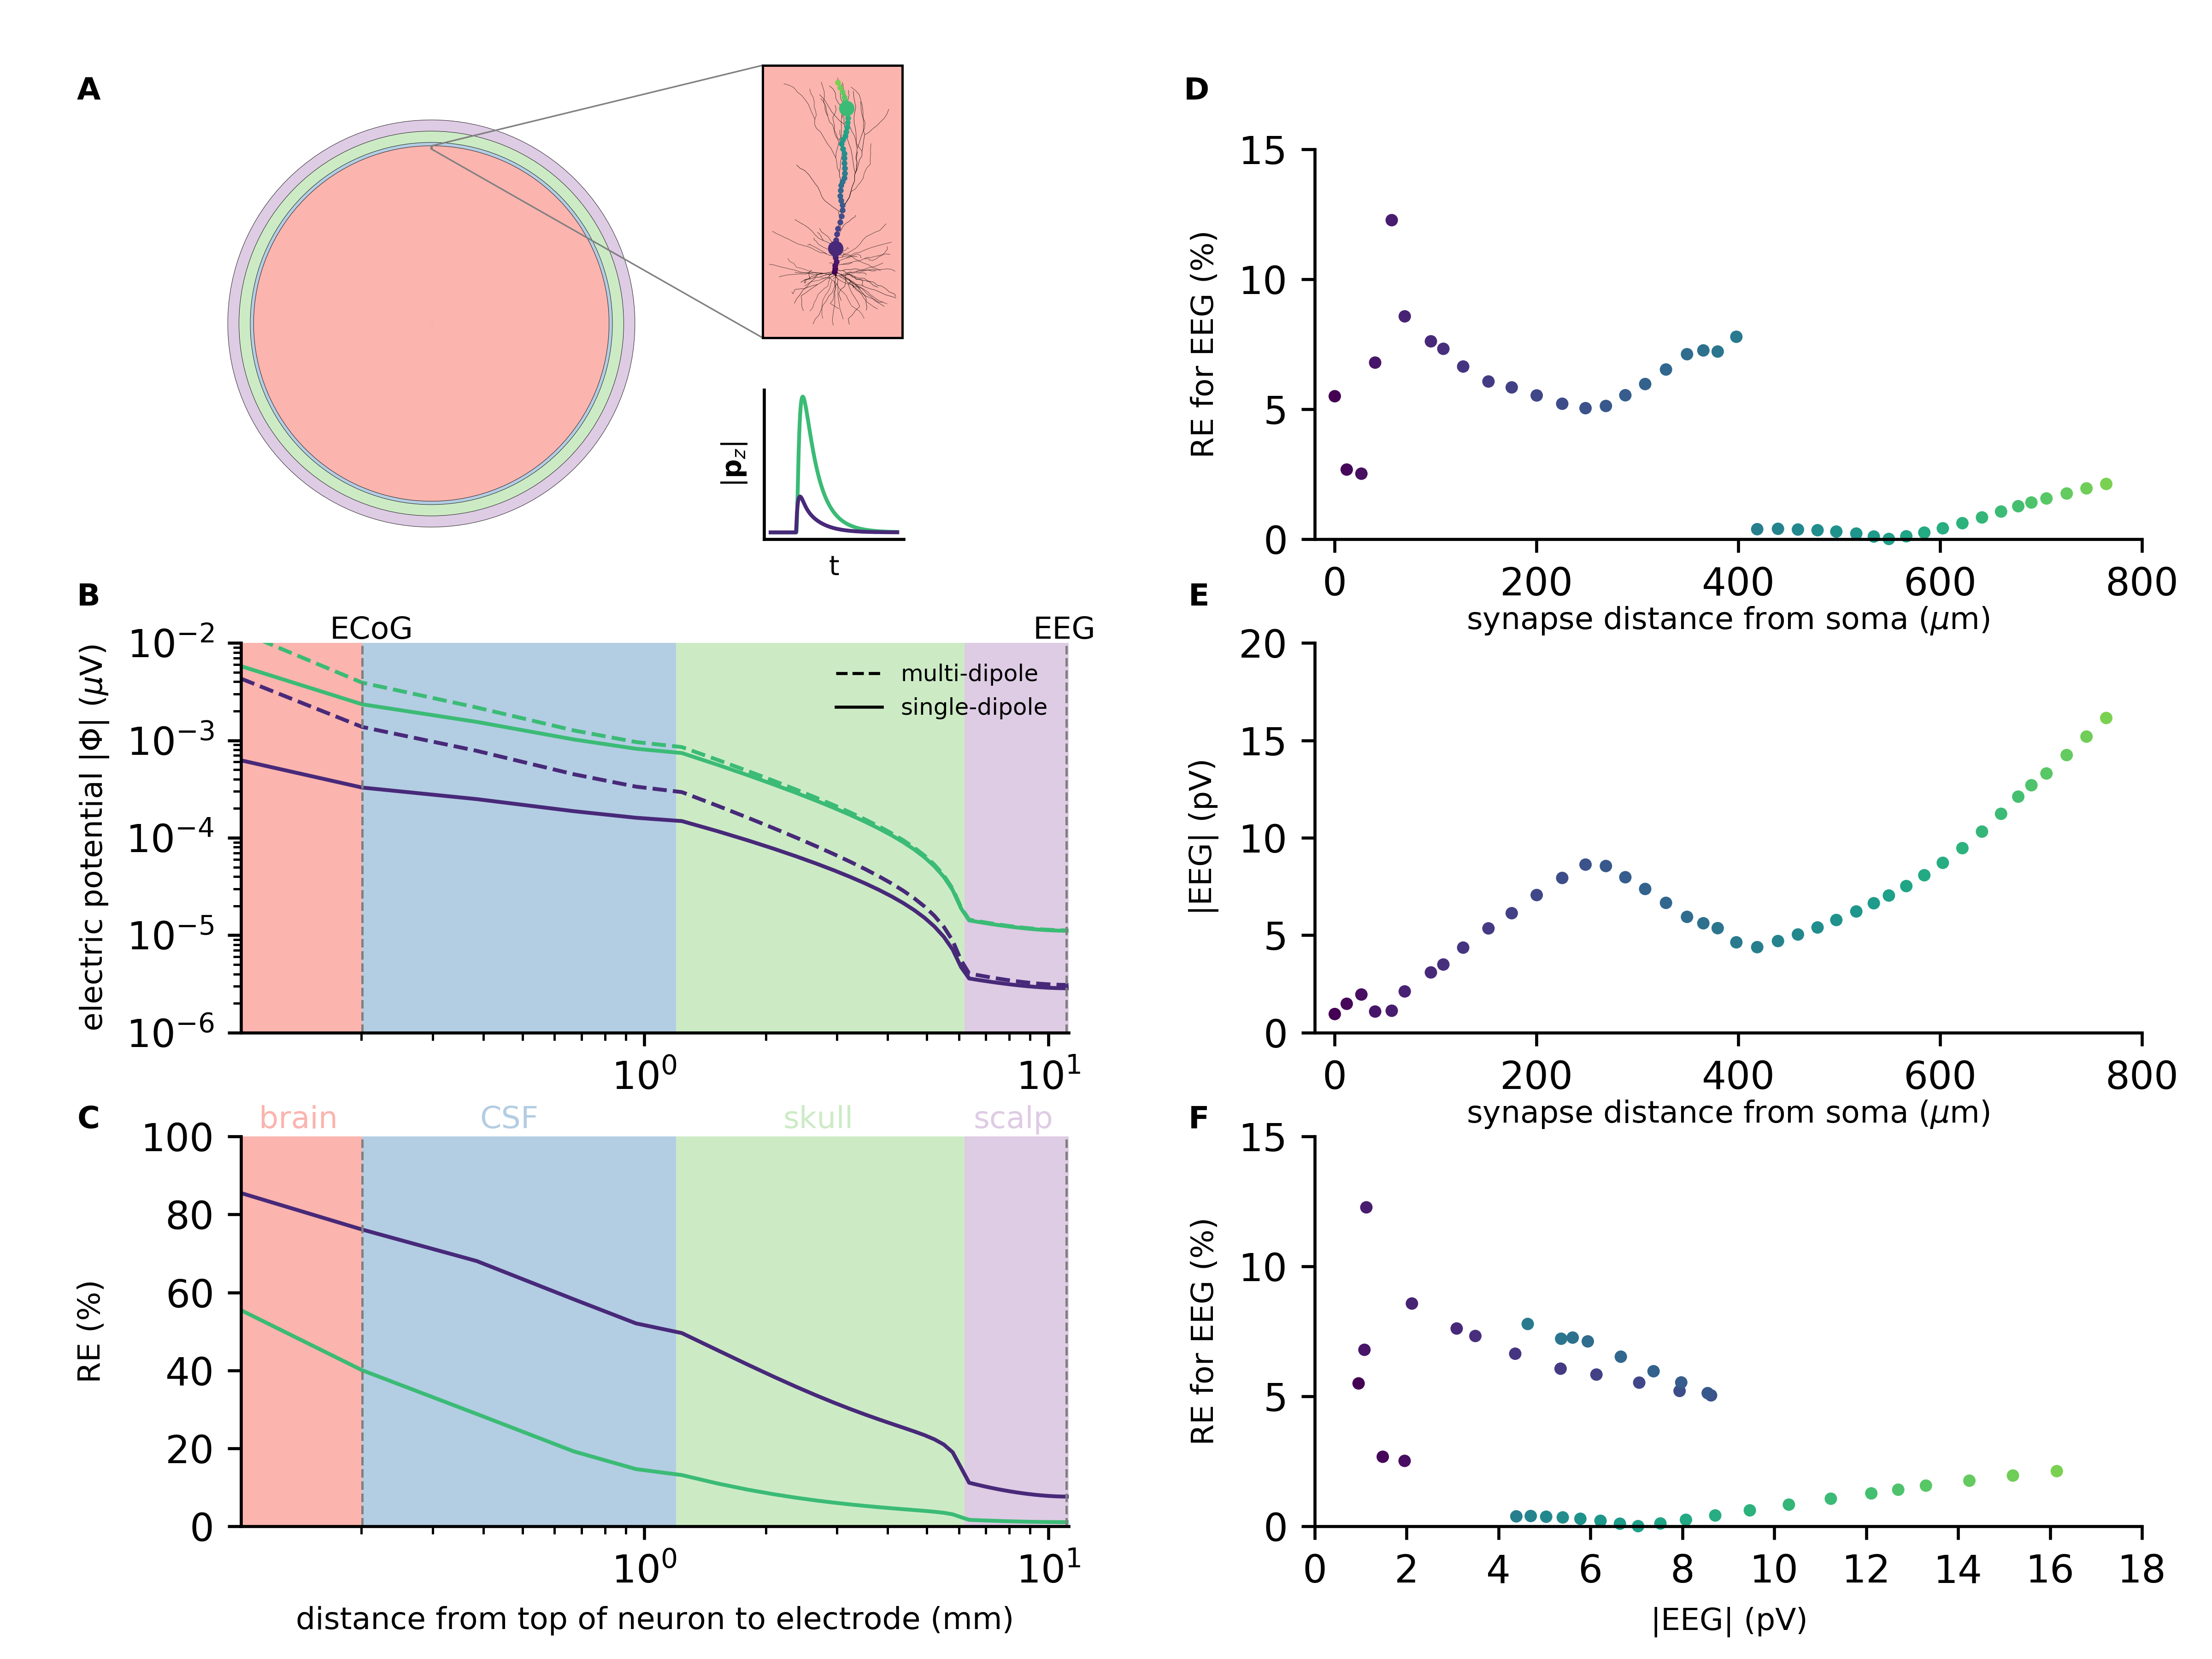
\includegraphics[width=1.0\textwidth]{figure2_eeg.png}
	\caption{\textbf{Single-dipole approximation is justified for EEG but not ECoG signals}. 
		\textbf{A}: Illustration of four-sphere head model, where the pink, blue, green and purple spherical shells represent the brain, CSF, skull and scalp respectively, see Table~\ref{tab:4sphere}. The pink inset shows the human layer-2/3 neuron \citep{EYAL2016} \sntxt{located in the brain, $78.9$~\si{mm} above head center}. $41$ simulations lasting 100 ms with a single synaptic input after 20 ms to cell with passive ion channels only, were performed for varying input locations, see colored dots. %\gen{100 ms er vel unodvendig lenge hvis man kun er ute etter max-amplituden?}
		The $z$-component of the resulting current dipole moments for two synaptic input locations (large colored dots) are shown in inset below as functions of time. The data presented in this figure are computed at the simulation time points producing the largest current dipole moment for each synaptic input location.
		\textbf{B}: Magnitude of extracellular potential $|\phi|$ as function of distance from the top of the neuron, shown for two simulations with synaptic input locations marked by large colored dots in upper inset of A. In each simulation, we consider the time point with the largest current dipole moment. Dashed lines show extracellular potentials computed with multi-dipole, and full lines show single-dipole calculations.
		%\tvnnote{Is the potential at a given timestep, or is it max? Should be mentioned here I think.}
		\textbf{C}: Relative error RE at EEG location comparing the single-dipole model to the multi-dipole model, as function of distance from top of neuron to measurement point.
		\textbf{D}: Relative error RE showing how single-dipole model deviates from multi-dipole model EEG calculations, as function of distance from soma to synapse location.
		\textbf{E}: Magnitude of EEG signal, $|\text{EEG}|$, as function of distance from soma to synaptic input location.
%		\tvnnote{Hadde det kanskje egentlig gitt mer mening å plotte EEG amplitude her? Kanskje mer ryddig å vise (enklere å forklare) at feilen i EEG-signalet er omvent korrelert med EEG amplitude?}
		\textbf{F}: Relative error, RE, showing how EEG calculations performed with the single-dipole approximation deviates from multi-dipole approach as a function of amplitude of the EEG signal, $|\text{EEG}|$.
		\gen{Fin figur, men jeg tror noe av skriften boer gjoeres litt stoerre. Og den fargede teksten i panel C er litt svak og vanskelig aa se.}
%		\gen{Siden vi nevner spesifikke tall (prosenter) for avvik i teksten, saa synes jeg tallene til denne hjernemodellen maa spesifiseres i detalj, kanskje i Methods? Dessuten boer vi nevne presist hvilken posisjon soma har.} 
		\gen{Kanskje vi kunne hatt enheter paa y-aksen i inset i A? Og det skal vel vaere $p_z$ ikke $\mathbf{p}_z$?}
		\snnote{Ok?}
		%		\tvnnote{Kanskje du kan skrive navnet på de forskellige regionene med tilhørende farge over panel C eller noe slikt? }
		%	\tvnnote{Suggestion: How about running another simulation with all synapses active simulataneously, calculate the relative error, and add it to this panel (F) as a horizontal line? We would expect this to give a small error, helping to illustrate our point of the EEG being dominated by low-error dipoles.}
	}
	%	\tvnnote{Suggestion: How about running another simulation with all synapses active simulataneously, calculate the relative error, and add it to this panel (F) as a horizontal line? We would expect this to give a small error, helping to illustrate our point of the EEG being dominated by low-error dipoles.}
	\label{fig:compare_multi_single_dipole}
\end{figure}

\subsection{Single-dipole approximation simplifies estimate of EEG contribution}\label{subsec:compare_neurons}
In the previous section, we showed that the single-dipole approximation was applicable for calculation of EEG signals, and in this section we demonstrate that the single-dipole approximation can substantially simplify the analysis of the biophysical origin of EEG signals.

Pyramidal cells have a preferred orientation along the depth axis of cortex (here the $z$-axis), and the direction of the current dipole moment $\mathbf{p}$ can be expected to align with this axis since
radial symmetry will tend to make the orthogonal components ($p_x$, $p_y$) cancel \citep{HAGEN2018}. 
%\gen{Boer det ikke vaere italic, dvs $p_x$, $p_y$?}
In contrast, interneurons show much less of a preferred orientation, and are therefore expected to give a negligible contribution to the EEG signal, except indirectly through synaptic inputs onto pyramidal cells \citep{HAGEN2016}.
We illustrated this by applying the single-dipole approximation to three different cell types (Fig.~\ref{fig:eeg_compare_cell_types}\textbf{A}), each receiving a large number of synaptic inputs with target regions on the cells set up to vary over time (Fig.~\ref{fig:eeg_compare_cell_types}\textbf{B}).

For the previously used human layer-2/3 cell (Fig.~\ref{fig:eeg_compare_cell_types}\textbf{A}, purple; \cite{EYAL2016})
receiving a volley of excitatory synaptic inputs that were restricted to the uppermost 200~$\si{\um}$ of the cell (time=50~ms; Fig.~\ref{fig:eeg_compare_cell_types}\textbf{B}, purple dots), we observed a negative deviation of $p_z$ (Fig.~\ref{fig:eeg_compare_cell_types}\textbf{C}, purple line). For basal synaptic input (time=100~ms; Fig.~\ref{fig:eeg_compare_cell_types}\textbf{B}, purple line), the polarity of $p_z$ was instead positive, but of slightly lower amplitude than for apical input, as can be expected because the large area of the somatic region will cause strong return currents in the immediate vicinity of the synaptic inputs, and therefore an overall weaker current-dipole moment.


A uniform distribution of 400 synaptic inputs across the cell membrane with area-weighted probability (time=150~ms; Fig.~\ref{fig:eeg_compare_cell_types}\textbf{B}, purple line), only gave rise to small ripples in $p_z$, due to the substantial cancellation of current dipoles of opposite polarity. It is sometimes assumed that excitatory input is relatively uniformly distributed onto pyramidal cells, while inhibitory input is more directed to the perisomatic region \citep{Mazzoni2015, Telenczuk2019, Skaar2020, Telenczuk2020}. As expected, we found that this combination of uniformly distributed excitatory synaptic input and perisomatic inhibitory input gave rise to a clear negative response in $p_z$ (time=200~ms; Fig.~\ref{fig:eeg_compare_cell_types}\textbf{B}, purple line), which could be part of the explanation why inhibitory synaptic input in some cases has been found to dominate the LFP \citep{HAGEN2016, TELENCZUK2016}.

For a rat cortical layer-5 pyramidal cell model (Fig.~\ref{fig:eeg_compare_cell_types}\textbf{A}, blue; \cite{HAY2011}), the resulting current dipole moment was very similar in shape, but larger in amplitude, which was expected because the longer apical dendrite will tend to give larger current dipole moments (Fig.~\ref{fig:eeg_compare_cell_types}\textbf{C}, blue line).
Lastly, we used a rat cortical layer-5 interneuron model (Fig.~\ref{fig:eeg_compare_cell_types}\textbf{A}, green; \cite{MARKRAM2015}), but since the dendrites of interneurons are not structured into the same distinctive zones as pyramidal cells, the synaptic input caused very small net current dipole moments.

We calculated the EEG signals with the four-sphere head model, using both the multi-dipole (Fig.~\ref{fig:eeg_compare_cell_types}\textbf{D}, dotted lines) and the single-dipole (Fig.~\ref{fig:eeg_compare_cell_types}\textbf{D}, solid lines) approach.
\tvntxt{To compare the approaches, we computed the relative error, as the absolute difference between the results from the two approaches, normalized by the maximum EEG magnitude computed with the multi-dipole approach.}
The single-dipole approach gave a maximum 
%\gen{"global error" maa forklares} 
error of  2.2$\%$, 3.5$\%$ and 0.34$\%$ for the human layer-5 cell, the rat layer-5 cell and the rat interneuron, respectively.
%\sout{In all three cases, we found the single-dipole approximation to be in excellently agreement with the multi-dipole approach, demonstrating that}  
%\sntxt{The resulting EEG signals modeled with the four-sphere head model is shown in Fig.~\ref{fig:eeg_compare_cell_types}. We applied both the multi-dipole (dotted line) and the single dipole model (solid line).} \snnote{maximum global error is 1.5$\%$ for Segev, 2.7$\%$ for Hay and 49$\%$ for interneuron. Don't know if we should include these numbers. It seems like these maximum errors occur for apical input, while in fig. 2 the largest errors followed basal input..}
%Note that in all cases, 
Importantly, the EEG signal is essentially fully described by the $z$-component of the current dipole moment $p_z$, that is, a single time-dependent variable. This reduction in signal description represents a massive simplification in the understanding of the biophysical origin of the EEG signal, compared to considering the transmembrane currents and position of each cellular compartment. 


\begin{figure}[H]
	\centering
	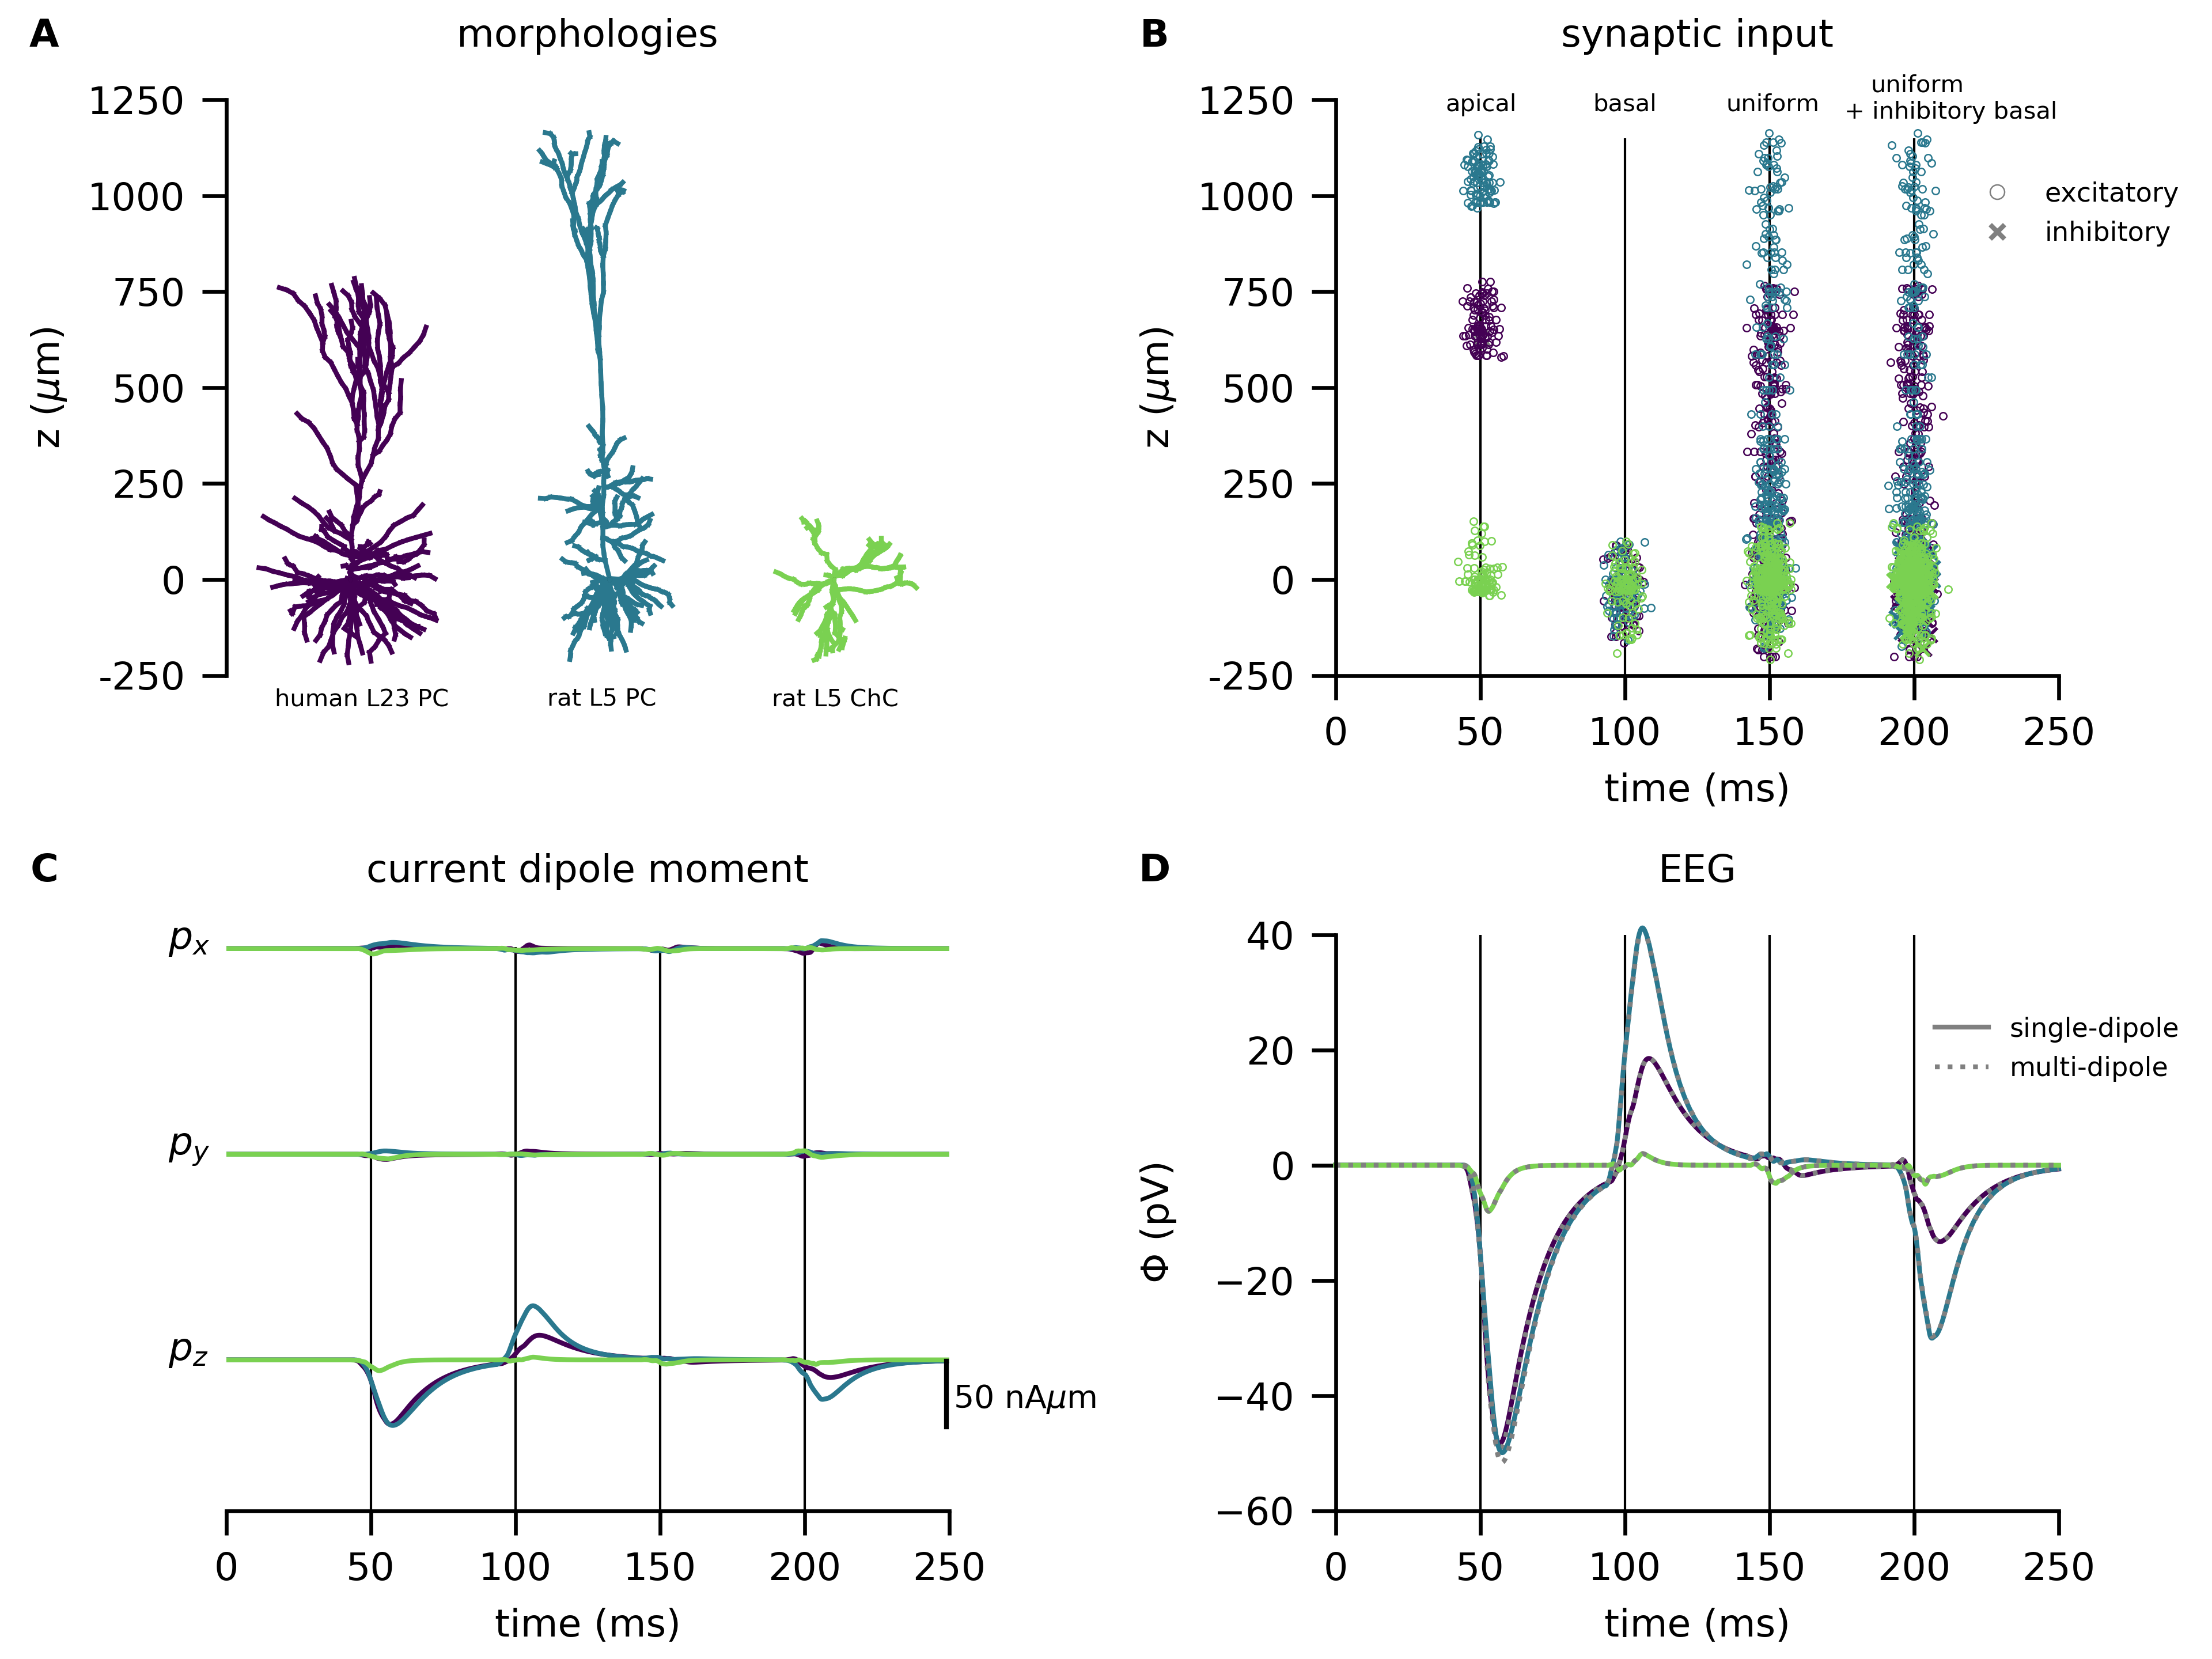
\includegraphics[width=1.\textwidth]{figure3.png}
	\caption{\textbf{EEG signals and current dipole moment from three different cell types with various synaptic input}.
		\textbf{A}: The morphologies of a human L2/3 pyramidal cell (purple; \cite{EYAL2016}), a rat L5 pyramidal cell (blue; \cite{HAY2011}), and a rat L5 interneuron (green; \cite{MARKRAM2015}). The remaining panels display data connected to each cell type, see cell-specific colors.
		\textbf{B}: Each dot represents an excitatory synaptic input at a specific time (x-axis) at a specific height of the neuron (z-axis, corresponding to panel A) for a specific cell type (color). The crosses mark inhibitory synaptic input. The four input bulks represent 1) 100 apical excitatory synapses, 2) 100 basal excitatory input, 3) 400 homogeneously spread-out excitatory synapses and 4) 400 homogeneously spread-out excitatory synapse and inhibitory basal synapses. The synaptic weights sum to 0.01~\si{\mu S} for all sets of excitatory/ inhibitory synapses in each wave. For the interneuron, which doesn't have typical "apical" or "basal" zones, the synapses were spread out all over the morphology for all input types.
		\textbf{C}: The x-, y- and z-components of the current dipole moment $\mathbf{p}$ for the three different cell types.
		\textbf{D}: EEG signals, $\phi$ from the three cell types computed with the four-sphere model.
		\gen{Synes spesifikasjon av synaptisk stroem maa vaere med et sted.}
		\snnote{Spesifisert i metode og i figurteksten til Fig. 1. Ok?}
%		\tvnnote{Nevne hvordan det er gjort for internevronet som ikke har apic og basal?}
%		\snnote{Har prøvd litt forskjellige løsninger her, men fant ut at det greieste var å ikke gjøre forskjell på apical/basal/uniform.}
	}
	\label{fig:eeg_compare_cell_types}
\end{figure}


\subsection{Current dipole moment expose dendritic calcium spikes}

\gen{Jeg synes dette er et veldig fint resultat som kanskje kan loeftes frem enda mer i artikkelen? Kanskje egen subsection? Og kanskje litt mer utbrodering av konklusjonen, dvs. hvorfor EEG signaler fra Ca-spikes vil dominere EEG-signaler fra aksjonspotensialer? Men jeg stusser litt paa amplituden 200 muA mum er jo gigantisk i forhold til Potjans-Diesmann nettverket som har pz mindre enn 100 nA mum.}


\cite{SUZUKI2017} recently demonstrated that dendritic calcium spikes can be recorded at the cortical surface, and that the signal amplitudes can be similar to contributions from synaptic inputs.

This demonstrates that active conductances may play an important role in shaping ECoG and EEG signals. Furthermore, it suggests that information about calcium dynamics might be present in such signals, and that this information could potentially be taken advantage of when studying learning mechanisms associated with dendritic calcium spikes \citep{SUZUKI2017}.
%\tvntxt{\sout{We found that the single-dipole approximation provides a convenient way of investigating the EEG-contribution \sntxt{\sout{of} from} such dendritic calcium spikes.}}

The previously introduced rat layer-5 cortical pyramidal cell model from \cite{HAY2011} can exhibit dendritic calcium spikes.
When this cell model received a single excitatory synaptic input to the soma (Fig.~\ref{fig:ca_spike}\textbf{A}, blue dot), strong enough to elicit a somatic action potential (Fig.~\ref{fig:ca_spike}\textbf{B1}, blue), a small depolarization was also visible in the apical dendrite (Fig.~\ref{fig:ca_spike}\textbf{B1}, orange). Even so, this did not initiate any dendritic calcium spike. However, when combining the same somatic synaptic input with an additional excitatory synaptic input to the apical dendrite, 400~$\si{\um}$ away from the soma (Fig.~\ref{fig:ca_spike}\textbf{A}, orange dot), we observed a dendritic calcium spike. This calcium spike did, in turn, induce two additional somatic spikes (Fig.~\ref{fig:ca_spike}\textbf{C1}).
For both synaptic input strategies described above, the extracellular potential simulated 30~$\si{\um}$ away from the soma took the shape of stereotypical extracellular action potentials: that is, a sharp negative peak followed by a broader and weaker positive peak (Fig.~\ref{fig:ca_spike}\textbf{B2, C2}). Further, we observed that the slow dendritic calcium spike was not reflected in the extracellular potential close to the soma (Fig.~\ref{fig:ca_spike}\textbf{C2}).
We found that for the case with only a somatic spike and no calcium spike, the single-cell current dipole moment resembled the inverse of the extracellular potential (Fig.~\ref{fig:ca_spike}\textbf{B3}), while for the case with both somatic and dendritic spiking, a pronounced slow component was also present in the single-cell current dipole moment (Fig.~\ref{fig:ca_spike}\textbf{C3}).
\tvntxt{\sout{Note that s}S}omatic action potentials are typically not expected to contribute significantly to EEG signals (but see \cite{TELENCZUK2015}), because the very short duration of spikes with both a positive and a negative phase implies that extreme synchrony is needed for spikes to sum constructively\tvntxt{, and spikes that are only partially overlapping tend to sum destructively. The same can not be expected to hold for the calcium spikes, which predominately cause a negative response in the current current dipole moment}. 
\tvntxt{To mimic a neural network scenario with multiple cells spiking at slightly different times, we calculated the sum of 1000 instances of the single-cell current dipole moment that was jittered (shifted) in time (normally distributed, standard deviation=10~ms).
We found that the case with the dendritic calcium spike had a $6.6$-fold larger maximum amplitude than the case with
only the somatic spike (Fig.~\ref{fig:ca_spike} \textbf{B4} versus \textbf{C4}, 
$\mathrm{max}|\mathbf{p}$| = 30.8~$\si{\uA}\cdot\si{\um}$ and 204.2~$\si{\uA}\cdot\si{\um}$ respectively).}
%\snnote{It is hard to read these numbers out from the plots.. Something odd with the axes here?}
\gen{Synes det boer sies litt klarere ett sted at "jittered"-effekten er en nettverkseffekt.} \tvnnote{OK?}
This demonstrates that dendritic calcium spikes are much more capable of summing constructively for a population of cells, and substantiates the role of dendritic calcium spikes in affecting ECoG/EEG/MEG recordings. 

\tvntxt{The amplitude of the slow component of the current dipole moment from the calcium spike was about 0.5~$\si{\uA}\cdot\si{\um}$ (Fig.~\ref{fig:ca_spike}\textbf{C3}), and later (Sec.~\ref{subsec:populations}) we will present results from a simulated neural network where the average event-related current dipole moment of layer 5 pyramidal cells were found to be about 0.1~$\si{\uA}\cdot\si{\um}$ (Fig.~\ref{fig:population}{\bf D}, bottom left). This indicates that our results are compatible with the claim by \cite{SUZUKI2017} that signal amplitudes from calcium spikes could be similar in amplitude to contributions from synaptic input.
}

\tvnnote{1 $\mu$A * $\mu$m ~-> 1 nV, so 10000 Ca spikes gives ~10 $\mu$V EEG.} 


It might initially seem surprising that the dendritic calcium spike is so strongly reflected in the single-cell current dipole moment, given that the transmembrane currents associated with the somatic action potential are much larger than those associated with the dendritic calcium spike: the maximum amplitude of the transmembrane currents of the somatic compartment was 45.1~$\si{\nA}$, compared to just 0.30~$\si{\nA}$ for the compartment in the apical dendrite (Fig.~\ref{fig:ca_spike}{\bf A}, blue and orange dots). 
\gen{Blir denne sammenligningen illustrativ naar det er saa stor forskjell paa arealet kompartmentene?} 
\tvnnote{Ikke helt sikker på hva du mener her?}
\gen{Og er ikke den storste stroemmen i akkurat disse kompartmentene den fra de synaptiske inputstroemmen og ikke en returstroem?} \tvnnote{I begge tilfeller er nok største strøm som følge av spikene, som kanskje er litt illustrert i B1 og C1, der vi ser at membranpotensialet først å fremst reflekterer spikes, og ikke synaptisk input. Bør vi utbrodere mer her?}
However, the current dipole moment is given as the product between the amplitude of the current and the separation between the source and sink ($\mathbf{p}=I\mathbf{d}$; Equation \ref{eq:dip_sum_axial}), and while the currents associated with the somatic action potential will for the most part be contained within the somatic region, giving very small sink/source separations, the currents associated with the dendritic calcium spike will be distributed over a much larger part of the cell membrane.
\tvntxt{This effect can be illustrated by comparing the spatial profile of the extracellular potentials around the neuron at a snapshot in time during a somatic spike or during a calcium spike (Fig.~\ref{fig:ca_spike} {\bf D} versus {\bf E}).}

\begin{figure}[H]
	\centering
	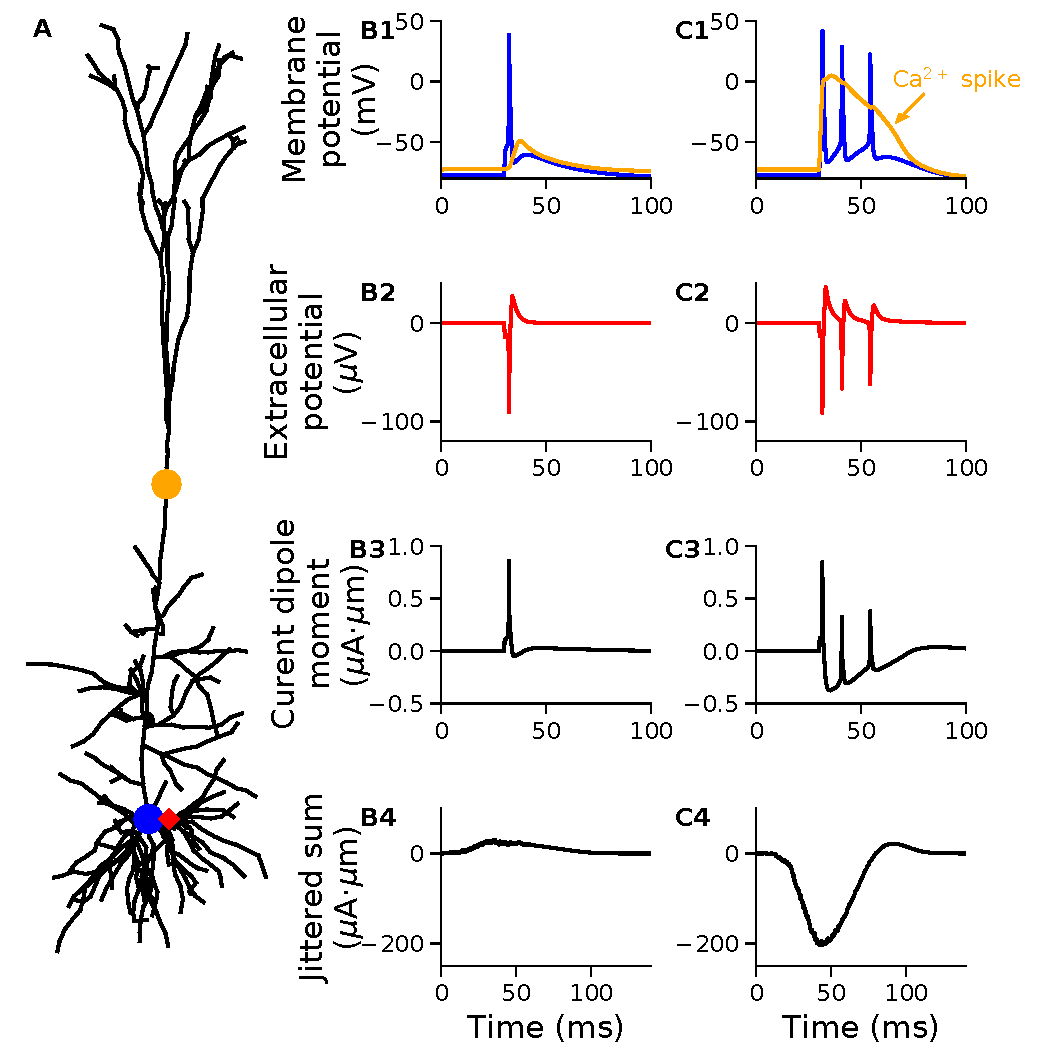
\includegraphics[width=0.6\textwidth]{ca_spike_hay}
	\caption{\textbf{Current dipole moment expose dendritic calcium spikes.}
		\textbf{A}: Layer 5 cortical pyramidal cell model from rat \citep{HAY2011}, receiving either a single excitatory synaptic input to the soma evoking a single somatic action potential (blue dot, results in \textbf{B1-4}), or in addition an excitatory synaptic input to the apical dendrite, evoking a dendritic calcium spike and two additional somatic spikes (orange dot, results in \textbf{C1-4}). 
		\textbf{B1, C1}: Membrane potential at the two positions indicated in \textbf{A}.
		\textbf{B2, C2}: Extracellular potential 30~$\si{\um}$ away from the soma (red diamond in \textbf{A}), assuming for illustration an infinite homogeneous extracellular medium. 
		\textbf{B3, C3}: Single-cell current dipole moment. 
		\textbf{B4, C4}: Sum of 1000 instances of the single-cell current dipole moment (from \textbf{B3, C3}), that has been randomly shifted in time with a normally distributed shift with a standard deviation of 10~ms. 
\tvntxt{\textbf{D:} Contour lines of extracellular potential around neuron at a snapshot in time during the somatic spike in \textbf{B1} (T=32.2~ms; time marked by dashed line).
\textbf{E:} Contour lines of extracellular potential around neuron at a snapshot in time during the calcium spike in \textbf{C1} (T=36.0~ms; time marked by dashed line).
The synaptic weight was 0.07 and 0.15 $\mu$S for the somatic and apical input location respectively.
}
	}
	\label{fig:ca_spike}
\end{figure}

\subsection{EEG from large-scale neural network simulations}
\label{subsec:populations}
So far, we have only considered EEG contributions from single cells, but real EEG signals are expected to reflect the activity of hundreds of thousands to millions of cells \citep{NUNEZ2006, COHEN2017}. 
%There are several ongoing large-scale modeling efforts that seek to simulate neural activity at different levels of biological detail. 
Biophysically detailed modeling of large populations is still in its infancy \citep{EINEVOLL2019} and at present typically include ``only'' a few tens of thousands of biophysically detailed cells \citep{MARKRAM2015, BILLEH2019}. Networks of point neurons, on the other hand, are regularly used to simulate hundreds of thousands \citep{BILLEH2019} or even millions of cells \citep{SENK2018, SCHMIDT2018}, but point-neurons lack the ability to predict LFP, ECoG, EEG or MEG signals \citep{EINEVOLL2013REVIEW}.  
To investigate EEG signals generated by neuronal networks, we therefore used a hybrid scheme \citep{HAGEN2016, SENK2018, Skaar2020}, where the network activity is first simulated in a highly computationally efficient manner with point neurons in NEST \citep{NEST} and the resulting spiking activity of each neuron saved to file. Afterwards, each cell is modeled with biophysically detailed multicompartment morphologies and the stored spikes of all the presynaptic neurons are used as synaptic input onto these neurons in a second simulation  where the extracellular potentials are calculated \citep{HAGEN2016, SENK2018}.

We used the large-scale point-neuron cortical microcircuit model from \cite{POTJANS2014, HAGEN2016}, which has $\sim$80 000 neurons divided into 8 different cortical populations, one excitatory and one inhibitory, across four layers (L2/3 - L6), and can exhibit a diverse set of spiking dynamics including different oscillations and asynchroneous irregular network states \citep{HAGEN2016, BRUNEL2000}. 
The only difference from the original simulations by \cite{HAGEN2016} was the added calculation of current dipole moments and EEG signals.
We simulated transient thalamic synaptic input to layers 4 and 6 (Fig.~\ref{fig:population}\textbf{A}), and after the spikes had been mapped onto the multicompartment cell models (Fig.~\ref{fig:population}\textbf{B}), we calculated the LFP (Fig.~\ref{fig:population}\textbf{C}) similarly to \cite{HAGEN2016} (their Fig.~1), in addition to the current dipole moments of each cell.

For all cell populations, we found that the current dipole moments from individual cells could show large transient responses to thalamic input (Fig.~\ref{fig:population}\textbf{D}; gray lines show current dipole moment from individual cells in two example populations: L5 inhibitory (L5I) and L5 exitatory (L5E)), but for all inhibitory populations the thalamic response was not visible in the average current dipole moment (Fig.~\ref{fig:population}\textbf{D}; black lines, L5I). The same was true for the current dipole moment components perpendicular to the depth axis for excitatory populations (Fig.~\ref{fig:population}\textbf{D}; L5E, $p_x$, $p_y$, black lines), but not for the component along the depth axis which had a substantial average response to the thalamic input (Fig.~\ref{fig:population}\textbf{D}; L5E, $p_z$, black line). 
These observations imply that, as previously noted, only the $z$-component of the current dipole moment from excitatory populations can be expected to contribute significantly to the EEG signal.

Our findings invite a simplified approach to calculate the EEG signal: Instead of calculating all single-cell EEG contributions and summing them (taking into account the position of the individual cells, similarly to what is done for the LFP signal), we can compute a single summed $p_z$-component from all neurons in each pyramidal cell population, place it in the population center, and calculate the resulting simplified EEG signal. This approximation is reasonable when the population radius is small compared to the distance from the population center to the EEG electrode. Note that the distance from the top of cortex to the top of the head is typically $\sim$10~mm, while the radius of the present simulated population is only 
$\sim$0.5~mm (Fig.~\ref{fig:population}; population outline in \textbf{B} is drawn in red in \textbf{E}).
Indeed, when we combined the current dipole moments with the four-sphere head model (Fig.~\ref{fig:population}\textbf{E}), we found that the full EEG signal that was calculated as the sum of the EEG contribution from each of the $\sim$80 000 cells at their respective positions, was in fact indistinguishable from the simplified EEG signal (Fig.~\ref{fig:population}\textbf{F}). This implies that the EEG signal from the simulated cortical activity can be fully represented by a single time-dependent variable for each pyramidal cell population.

We also compared the relative amplitude of the EEG signal from each population, and found that for the present example, the excitatory population of L2/3 was the dominant source of the EEG signal (Fig.~\ref{fig:population}\textbf{F}). Note, however, that we expect this observation to be somewhat model-dependent, and that strong general claims about the contribution of different pyramidal cell populations to the EEG signal cannot be made from this example study alone.

\begin{figure}[H]
	\centering
	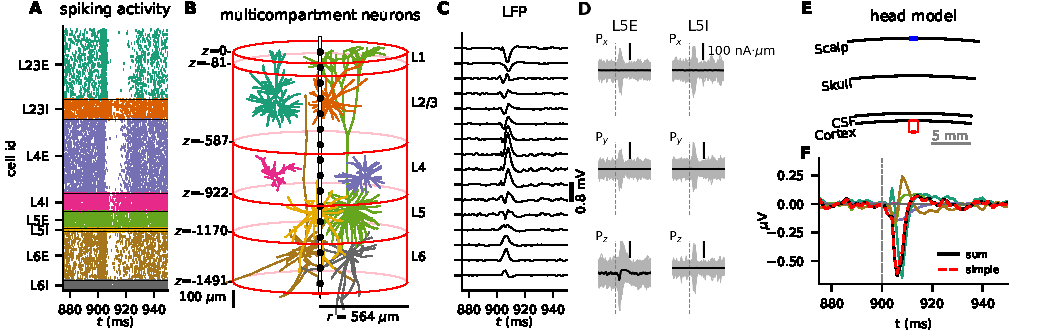
\includegraphics[width=1.0\textwidth]{hybrid_with_EEG}
	\caption{\textbf{Large-scale neural simulations can be used to probe biophysical origin of EEG signals}. 
		\textbf{A}: Stimulus-evoked spiking activity from thalamic input (time $t= $ 900~ms, denoted by thin vertical line) in the cortical microcircuit model from \cite{POTJANS2014}. Dots indicate spike times of individual neurons, and populations are represented in different colors (I=inhibitory, E=excitatory).
		\textbf{B}: Multicompartment model neurons used to produce the measurable signals, with colors corresponding to panel \textbf{A}, showing one example morphology per population. Layer boundaries are marked at depths relative to cortical surface, z = 0. A laminar recording electrode with 16 contacts separated by
		100 $\mu$m (black dots) is positioned in the center of the population.
		\textbf{C}: LFPs calculated at depths corresponding to black dots in \textbf{B}.
		\textbf{D}: For the two L5 populations (L5I and L5E), the three components of the current dipole moment is shown for all individual cells (gray), together with the population average (black).
		\textbf{E}: Illustration of the four-sphere head model, with the red column corresponding the the outline of the population in panel \textbf{B}.
		\textbf{F}: The EEG signal from each population found by summing the single-cell EEG contribution of all individual cells within each population (different colors, same color scheme as in \textbf{A},\textbf{B}), together with the total summed EEG signal (black). The simplified EEG signal was found by first summing the $z$-component of the current dipole moments for all pyramidal cells, that is L2/3E, L5E and L6E, and calculating the EEG from this single current dipole (red dashed).
	}
	\label{fig:population}
\end{figure}


\subsection{Dipole approximation in complex head models}
%The construction of such realistic head models are typically dependent on very expensive equipment, such as magnetic resonance imaging (MRI), to map the electrical conductivity of the entire head at resolutions of $\sim$0.5-1.0~mm$^3$ \citep{HUANG2015, HUANG2016}. Afterwards, numerical techniques such as the Finite Element Method (FEM) \citep{LOGG2012} can be used to calculate the signal at the EEG electrodes for arbitrary complex head geometries and arbitrary arrangements of current dipoles in the brain, but at a high computational cost.

Even though the four-sphere head model is convenient for generic EEG studies, many applications such as accurate EEG source analysis, may require more detailed head models \citep{DALE1999, VORWERK2014}.
%The four-sphere head model (Fig.~\ref{fig:compare_head_models}A) can be \sntxt{\sout{a}} convenient \sntxt{\sout{head model}} for some generic EEG studies, but for many applications more realistic head models will be needed \citep{DALE1999, VORWERK2014}. 
The construction of such complex head models is typically dependent on expensive equipment, %\snnote{MRI er vel det essensielle "expensive equipment" her, saa ville ikke tenkt paa MRI som et eksempel, men heller hovedutstyret? Isaafall ville jeg skrevet "that is" isteden for "such as". Eller er det andre dyrt utstyr som ogsaa er viktig?}
%\tvnnote{du har nok rett}
that is magnetic resonance imaging (MRI), to map the electrical conductivity of the entire head at resolutions of $\sim$0.5-1.0~mm$^3$
%\snnote{are these numbers relevant, or is it better to just say: "very high resolutions"?}
%\tvnnote{I think they are good :-)}
\citep{HUANG2015, HUANG2016}. Afterwards, numerical techniques such as the Finite Element Method (FEM) \citep{LOGG2012} can be used to calculate the signal at the EEG electrodes for arbitrary arrangements of current dipoles in the brain, but at a high computational cost.
%\snnote{vet ikke om det var dette du mente i neste setning.. Ble det oppklarende eller misvisende, synes du?} \tvnnote{bra sann det er naa :-)}
The number of computing hours is, however, reduced by applying the reciprocity principle of Helmholtz. The reciprocity principle states, in short, that switching the location of a current source and a recording electrode will not affect the measured potential \citep{Malmivuo1995, Ziegler2014, HUANG2016, Dmochowski2017}. %\gen{I 2.2.2 ble det kun referert til Rush og Driscoll, 1969 paa dette punktet.}
 This implies that it suffices to use FEM to calculate the lead field in the brain from virtual current dipoles placed at each of the EEG electrodes. From the lead field matrix, we can infer the potential at the EEG electrodes, given an arbitrary arrangement of current dipoles in the brain.
Luckily, %\gen{Juhu ... :-) Vanligvis oppfattes vel "Fortunately" som et mer serioest ord, men "by all means".}
several such pre-solved complex head models are freely available, and one example is the {\it New York Head} (NYH) (Fig.~\ref{fig:compare_head_models}\textbf{A}), which we have applied here (\cite{HUANG2016}; \url{www.parralab.org/nyhead/}).

%\snnote{Det neste avsnittet har jeg sett meg litt blind paa. Blir veldig glad for endringer/ innspill her!til hvordan folgende del skal bli bedre!}
%\tvnnote{I think it could be improved by writing about the two positions at the same time: ``To illustrate the use of pre-solved complex head-models, we calculated and compared the EEG signals resulting from the current dipole moment obtained in Section subsec:populations inserted into either the four-sphere or the NY head model.
%We show results for the current dipole being positioned in two different brain regions of the NY head model, namely .... In both cases the current dipole moment was oriented along the depth axis of the cortex ... Note that because of the intrinsic complexity of the NY head model, the amplitude of the EEG signal is very different in the two cases, while it was much more similar for the four-sphere head model ...'' Maybe it is sufficient to give the distanced to the closest electrode only in the caption.}
%\snnote{Good idea!}

To illustrate the use of pre-solved complex head-models, we inserted the current dipole moment obtained in section~\ref{subsec:populations} into the New York Head model (Fig.~\ref{fig:compare_head_models}\textbf{A}), at two manually chosen positions: one in the parietal lobe, and one in the occipital lobe, see stars in Fig.~\ref{fig:compare_head_models}\textbf{C, E}, respectively.
	In both cases, the current dipole moment was oriented along the normal vector of the brain surface, and the EEG signal was calculated.
\sntxt{For comparison with a simplified head model, we inserted the same current dipole moment into the four-sphere head model  (Fig.~\ref{fig:compare_head_models}\textbf{B}) at locations comparable to the dipole positions chosen in the occipital and parietal lobe in the NYH model: the locations in the four-sphere model were chosen close to the brain surface, such that the distance from dipole position to closest electrode (Fig.~\ref{fig:compare_head_models}\textbf{D, F}, stars) and the brain surface normal vectors were similar to the respective positions in the NYH model.}
%	We then found dipole positions in the four-sphere head model (Fig.~\ref{fig:compare_head_models}\textbf{B}) with the same brain surface normal vectors
%\gen{Hva menes her?}	
%	 and comparable distances to closest EEG electrode (Fig.~\ref{fig:compare_head_models}\textbf{D, F}, stars), and
% computed the EEG signal \sntxt{with the four-sphere model} from the same current dipole moment \sntxt{as for the NYH model}.
The computed EEG signals from the two head models were in this case relatively comparable in both spatial shape and amplitude (Fig.~\ref{fig:compare_head_models}\textbf{C-F}). The two head models also generated EEG signals of the same temporal shape, as expected, but while the four-sphere head model gave very similar EEG amplitudes for the two different dipole locations, the EEG amplitudes from the complex head model was much more variable, even for similar distances to the closest electrode (Fig.~\ref{fig:compare_head_models}{\bf G}, {\bf H}).

%\tvnnote{ikke sant? Har du avstandene?}
%\snnote{Ja! Parietal: 16.13mm i 4S og 16.76 i NYH.  Occipital: 16.90 mm i 4S og 14.64mm i NYH. Det som kanskje er litt dumt, er at der EEG-amplitudene for de to modellene ser mest sammenliknbare ut, dvs for dipol i occipital lobe er det 4S som har størst amplitude og lengst avstand fra dipol til nærmeste elektrode. Hvis avstanden hadde vært mer lik som i NYH ville altså ville vi hatt større forskjeller i amplitude for de to modellene.. Går det greit synes du, eller skal jeg gjøre et forsøk til på å flytte elektrodene i 4S-modellen, sånn at nærmeste elektrode kommer nærmere?}
The higher variability of the complex head model was also apparent in the decay of the maximum EEG amplitude with distance, which was perfectly smooth, exponential-like \citep{NUNEZ2006}, and very similar for the two locations in the four-sphere model, but very variable for the complex head model, although with the same general shape (Fig.~\ref{fig:compare_head_models}{\bf I}, {\bf J}). %\gen{Jeg synes ikke dette var aapenbart utfra figuren.}


%To illustrate the use of pre-solved complex head-models, we computed and compared EEG signals resulting from the current dipole moment obtained in Section~\ref{subsec:populations} inserted into the New York Head model (Fig.~\ref{fig:compare_head_models}\textbf{A}) and the four-sphere head model (Fig.~\ref{fig:compare_head_models}\textbf{B}). We show results for the current dipole being manually positioned in two different brain regions of the NYH model, namely the parietal lobe and the occipital lobe.

%In both cases the current dipole moment was oriented along the normal vector of the brain surface in the NYH model. Then, we found a comparable position in the four-sphere model, with the same brain surface normal vector \tvnnote{and comparable distance to closest EEG electrode?}. Further, we computed the resulting EEG signals applying the two head models as shown in Fig.~\ref{fig:compare_head_models}\textbf{C-F} for the time point of the population simulation giving with the largest current dipole moment amplitude ($t_{max}$). 

%\tvntxt{\sout{When looking at the EEG trace measured by the electrode closest to the dipole, we can see that t}T}he two \tvntxt{head} models generate \tvntxt{EEG} signals of the same shape, as expected (Fig.~\ref{fig:compare_head_models}{\bf G}, {\bf H}). Plotting the EEG signals at time point $t_{max}$ for all electrodes as a function of distance from current dipole moment to electrode, showed that the EEG signal decays exponentially with distance \tvnnote{Bortsett fra at den tilsynelatende begynner såvidt å øke igjen ganske fort (etter at den har krysset null?). Har du sjekket at det er exponentially} \citep{NUNEZ2006} (Fig.~\ref{fig:compare_head_models}{\bf I}, {\bf J}). Because of the intrinsic complexity of the NYH model, the amplitude of the EEG signal is very different for the two dipole positions. When applying the four-sphere model, on the other hand, the different dipole positions resulted in much more similar EEG amplitudes.

Note that despite the complexity, the NYH model is substantially faster than the four-sphere model. In order to simulate the EEGs from a dipole moment vector containing 1200 timesteps, the NYH model execution times were $\sim$~0.4~s, while the four-sphere model needed $\sim$~1.5~s.

\begin{figure}[H]
	\centering
	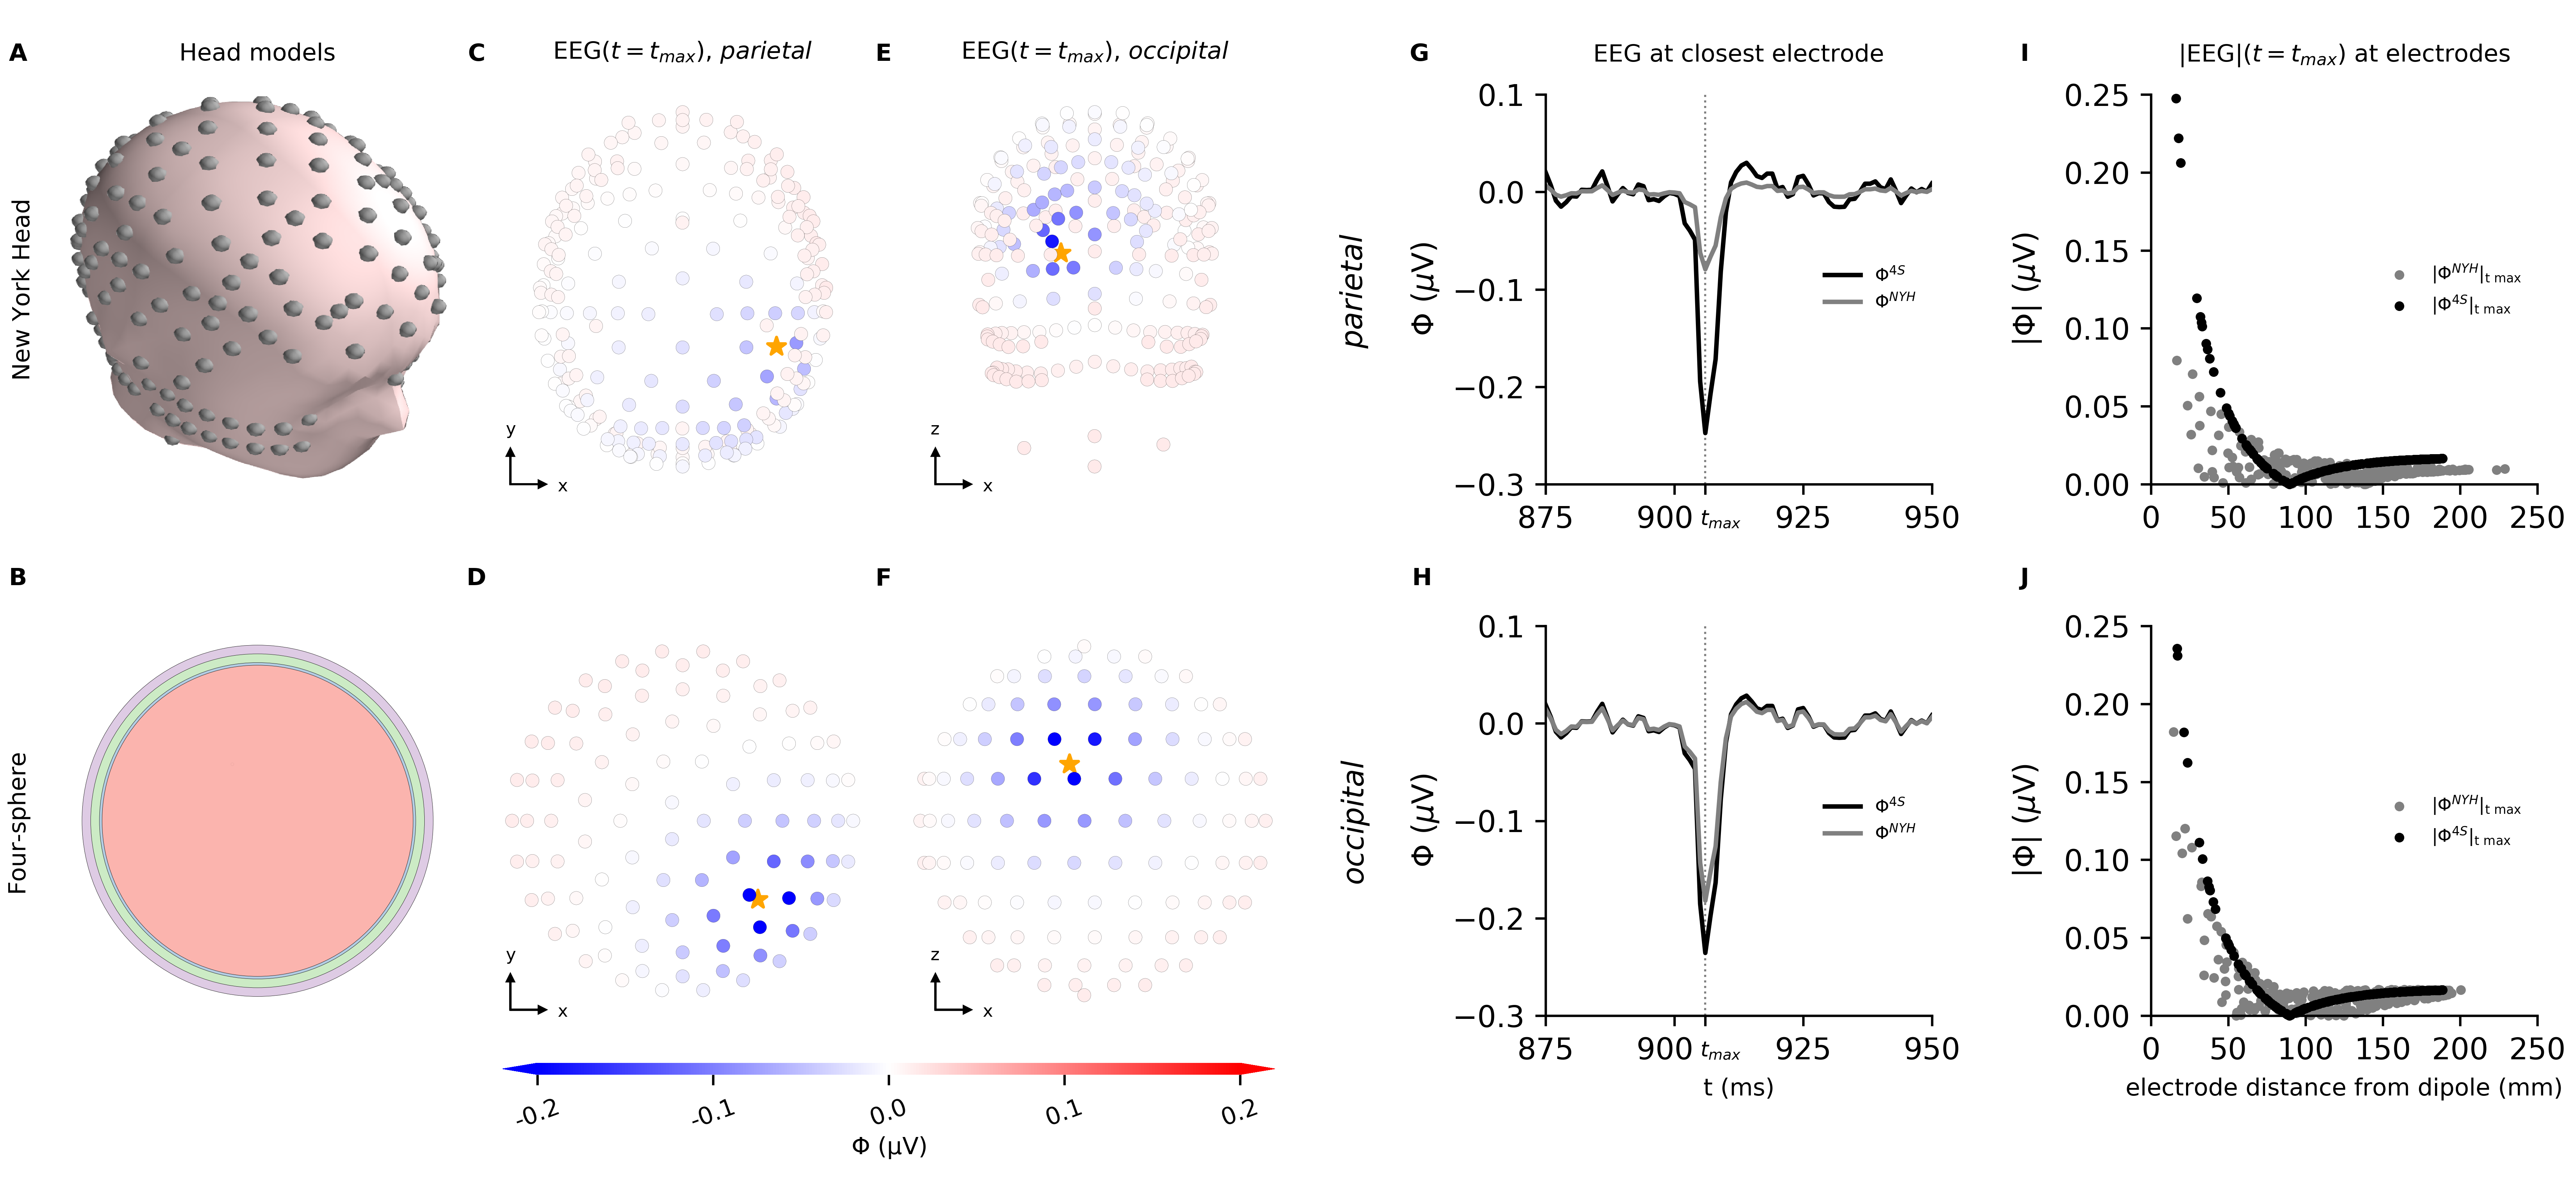
\includegraphics[width=1.0\textwidth]{figure6.png}
	\caption{\textbf{EEG signals from neuron population can be modeled with the four-sphere model and the New York Head}. EEG signals from population dipole resulting from waves of synaptic input to the cortical microcircuit model from \cite{POTJANS2014}. Population dipole was placed in two different locations: parietal lobe (C,D,E,F) and occipital lobe (G,H,I,J).
		{\bf A}: The four-sphere model consisting of four concentrical shells: brain tissue, CSF, skull and scalp.
		{\bf B}: The New York Head model.
		{\bf C, D}: EEG signals ($\phi$) on scalp surface electrodes, seen from above, showing time point of the strongest current dipole moment $|{\bf p}|$ of the population simulation. Dipole is placed in the parietal lobe and location is marked by orange star, having the following coordinates in the NYH model: (55, -49, 57)~mm. EEG signals were computed with the New York Head model (C) and the four-sphere head model (D).
		{\bf E}: EEG trace computed with the four-sphere model (black) and the New York Head model (gray) on closest scalp surface electrode: i.e. the electrode with the shortest distance to the current dipole moment location. Dipole is placed in parietal lobe (distance is 16.13~mm for the four-sphere model and 16.76~mm for NYH).
		{\bf F}: Absolute value of EEG signals from panel C,D generated by dipole in parietal lobe, plotted as function of distance from dipole to measurement electrode. 
		{\bf G,H}: Equivalent to panel C,D, however, dipole is placed in occipital lobe, and electrodes are seen from the back of the head. Dipole coordinates for NYH model: (-24.3, -105.4, -1.2)~mm.
		{\bf I}: EEG trace from dipole in occipital lobe computed on closest electrode (distance is 16.90~mm for the four-sphere model and 14.64~mm for NYH), equivalent to panel E.
		{\bf J}: Equivalent to panel F, with EEG signals from panel G,H generated by dipole in occipital lobe.
%		\snnote{will fix fonts of "parietal" and "occipital"}
		%	\snnote{The layout of this figure was meant to be pedagogical, as the rows, columns show the same model/ dipole location, but it's probably not compact enough..}
		%	\snnote{The same number of electrodes (224) in the four-sphere model for both dipole locations. Can try to optimize this, to get minimal distance between dipole and closest electrode.}
		%	\snnote{compute angle between EEG electrode and current dipole moment/ current dipole position vector. This should also affect the amplitude..}
%		\tvnnote{Kanskje egentlig litt like farger i G-J? Hva med svart og grå?}
%		\snnote{God idé!}	
	}
	\label{fig:compare_head_models}
\end{figure}

%\tvnnote{When we have a figure with a single current dipole of, say 1 nA/um, and corresponding EEG potentials, of say, 1 uV, we should send it to the New York Head model people (Stefan Haufe), and ask for a confirmation that the magnitude of the EEG in relation to the current dipole makes sense}
%%%%%%%%%%%%%%%%%%%%%%%%%%%%%%%%%%%%%%%%%%%%%%%%%%%%%%%%%%%%%%%%%%%%%%%%
%%%%%%%%%%%%%%%%%%%%%%%%%%%%%DISCUSSION%%%%%%%%%%%%%%%%%%%%%%%%%%%%%%%%%
%%%%%%%%%%%%%%%%%%%%%%%%%%%%%%%%%%%%%%%%%%%%%%%%%%%%%%%%%%%%%%%%%%%%%%%%
\section{Discussion}\label{sec:discussion}
%Order:
%summary
%
%EEG is important but little is known, this work lays foundation
%Easy to study contribution, decoupled from head model (like Ih or Ca)
%Source localization
%
%Sinlge cells and head models fairly well understood but not circuit level
%Hard, but several ongoing projects, like Allen and HBP, which we expect will be increasingly important in neuroscience over the comming years.
%Our work enables EEG from large scale sims in complex head models
%
%TVB and HNN are doing important and related work, but at somewhat different levels
%
%Our approach can be used to calculate mappings from firing rates to EEGs through the kernel method, thereby meeting TVB.
%
%A better understanding of EEG signals could lead to important discoveries (Mäki-Marttunen et al. 2019)
%Our approach should ideally be used in combination with animal studies (Bruynes-Haylett et al. 2017)

%\subsection*{Summary}

\subsection{Summary}
%\gen{Jeg synes ikke denne starten er helt optimal siden en kan faa inntrykk av at det "nye" allerede er brukt i to tidligere arbeider. Kanskje bedre med aa starte med aa fortelle om de nye testene og applikasjonene av approachen?}
In this paper, we have introduced an approach for reducing arbitrary simulated neural activity to single current dipoles (Fig.~\ref{fig:dipole_field}). 
%Note that we have implemented all methods into the open-source python tool LFPy 2.0 and that the exact implementation presented here has already been used by \cite{HAGEN2018} and \cite{MAKI2019}. 
We verified that the approach was applicable for calculating EEG, but not ECoG signals (Fig.~\ref{fig:compare_multi_single_dipole}-\ref{fig:eeg_compare_cell_types}), and gave examples of how reducing neural activity to a single dipole can be a powerful tool for investigating and understanding single-cell EEG contributions (Fig.~\ref{fig:eeg_compare_cell_types}-\ref{fig:ca_spike}). Furthermore, we demonstrated that the presented approach could easily be integrated with existing large-scale simulations of neural activity. Moreover, it was shown how single dipoles are useful for constructing compact representations of the EEG contributions from entire neural populations, with methods still firmly grounded in the underlying biophysics (Fig.~\ref{fig:population}). Finally, we demonstrated how the simulated current dipoles, from single cells or large neural populations, can be directly inserted into complex head models for calculating more realistic EEG signals (Fig.~\ref{fig:compare_head_models}).

\subsection{Application of current dipoles}
We have highlighted that the calculation of current dipoles from neural activity is cleanly separated from the calculation of the ensuing EEG signals. The same is true for MEG signals, and the calculated current dipoles can therefore also be used in combination with simplified or detailed frameworks for calculation of MEG signals, for example by following methods outlined by \cite{Ilmoniemi2019}.
For calculation of ECoG signals our results suggested that the single-dipole approximation gave substantial errors, and for simulations with multi-compartment neuron models it therefore seems advisable to use the standard compartment-based formalism, potentially in combination with the method of images \citep{Pettersen2006, HAGEN2018}.


\subsection{Generalization to non-compartmental models}
EEG and MEG recordings reflect neural activity at the systems-level \citep{Pesaran2018, EINEVOLL2019}. Here we have focused on calculating current dipoles from detailed multi-compartment neuron models, but neural modelling at the systems-level is often based on higher levels of abstractions, like point neurons \citep{NEST} or firing rate populations \citep{TVB}.
Calculation of electric or magnetic signals from such higher-level neural simulations must in general rely on some kind of trick, since neurons require a spatial structure to be capable of producing electromagnetic signals \citep{EINEVOLL2013REVIEW}.
One such trick that has already been taken advantage of here is the hybrid scheme, where neural network activity is first simulated by point neurons, and the resulting spike trains replayed onto multi-compartment neuron models for calculating LFP and EEG signals (sec.~\ref{subsec:populations}; Fig.~\ref{fig:population}). This can be further generalized by using the so-called kernel method, which has previously successfully been applied to the LFP \citep{HAGEN2016, Skaar2020, Telenczuk2020}. In practice, this would involve simultaneously activating all outgoing synapses from a simulated population, and recording the total current dipole moment of the response (the kernel) \citep{HAGEN2016}. Convolving this kernel with the population firing rate would then provide a good approximation of the current dipole moment caused by the given neural population, and the EEG/MEG contribution could subsequently be calculated.
This would enable calculation of EEG and MEG signals directly from point-neuron or firing-rate models, in a manner that is firmly grounded in the underlying biophysics. 
The calculated kernels would be valid for different kinds of input to the original network model, but would in general have to be recomputed for changes to cell or synaptic parameters. 
In many cases, it seems likely that kernels from neighboring neural populations will be similar, and if so, generalization to larger networks should be possible, without the need to construct biophysically detailed models of a corresponding size.
\tvnnote{Bør vi gå dypere inn i dette?}


\subsection{Connection to other work}
Calculation of current dipole moments from morphologically complex cell models has been pursued before, for example to study the EEG and MEG contribution of spiking single cells \citep{Murakami2006}, or to study how the synaptic input location affects the current dipole \citep{LINDEN2010, AHLFORS2015}.
Important work on EEG interpretation in terms of the underlying neural activity has also previously been done through use of "minimally sufficient" biophysical models, see for example \cite{Murakami2002, Murakami2003, Jones2007, Jones2009, Sliva2018, NEYMOTIN2020}. 
Here, "minimally sufficient" means that the cell models only had the minimum needed spatial structure (point neuron can not produce current dipole moments), only considered a few cell types, and employed simple synaptic connection rules.
In particular, the Human Neocortical Neurosolver (HNN) \citep{NEYMOTIN2020} enables researchers to link measured EEG or MEG recordings to neural activity through a pre-defined canonical neocortical column template network. 
HNN comes with an interactive GUI, designed for users with little or no experience in computational modeling, and might therefore be an appropriate choice for researchers seeking to gain a better understanding of their EEG/MEG data.  
However, while the use of such minimally sufficient models allows for quick and direct comparison between simulated and recorded EEG signals, it is not (presently) compatible with simulating EEG or MEGs from biophysically detailed single cell- or network models, constructed from detailed experimental data \citep{Reimann2013, Egger2014, MARKRAM2015, HAGEN2016, Gratiy2018, Arkhipov2018, BILLEH2019}.  

A more high-level approach to simulate MEG/EEG signals from the underlying neural activity has been pursued through neural field or neural mass models \citep{Jirsa2002, David2003, Coombes2006, Deco2008, Bojak2010, Ritter2013}, which aim to model the evolution of coarse-grained variables such as the mean membrane potential or the firing rate of neuron populations. Such coarse-graining drastically reduces the number of parameters and the computational burden of the simulation, and can be used to study the interplay among entire brain regions, and indeed run whole-brain simulations. 
The Virtual Brain (TVB) is an excellent example of a software for whole-brain network simulations \citep{TVB, Sanz-Leon2015, Ritter2013}, where detailed and potentially personalized head models can be combined with tractography-based methods identifying the connectivity between brain regions \citep{TVB}. To calculate measurement modalities like MEG and/or EEG signals from neural field or neural mass models, it is typically assumed that the population current dipole moments are roughly proportional to, for example, the average excitatory membrane potential \citep{Bojak2010, Ritter2013}. Further, EEGs can be calculated from the resulting current dipole moments in combination with head models as presented in this paper, or through other softwares or techniques \citep{Gramfort2014}.
This suggests an intriguing future development, where one could apply the previously described kernel method to substantially increase the accuracy of LFP, EEG and MEG predictions from high-level large-scale simulations of neural activity. 

\subsection{Outlook}
\tvnnote{De to første avsnittene her er flyttet hit fra forrige versjon, var ikke med i forslaget til Gaute. Hvis det blir for rotete eller for mye, er det selvfølgelig greit for meg å fjerne dette igjen :-)}
EEG signals have been an important part of neuroscience for a century, but still very little is known about the neural origin of the signal \citep{COHEN2017}. This work lays some of the foundation for obtaining a better understanding of the EEG signal, by allowing easy calculation of scalp potentials from arbitrary simulated neural activity.
The presented formalism is well suited for modeling EEG contributions from various potential neural origins,  including different cell types, different ion channels and different synaptic pathways. 
For example, to study the effect of calcium spikes \citep{SUZUKI2017}, I$_{\rm h}$ currents \citep{NESS2016, NESS2018, KALMBACH2018}, or gene expression on EEG signals \citep{MAKI2019b}, one only needs to know how the $z$-component of the resulting population current dipole is affected.
This decoupling of the current dipole moment and head model allows for easier investigation and improved understanding of the origin of the EEG signal.

EEG measurements are often used for source localization, aiming to identify the underlying cortical current dipoles \citep{NUNEZ2006, Gramfort2014, Ilmoniemi2019}. However, such reconstructed current dipoles are generic in the sense that they are typically not intended to represent specific neural populations. By allowing for calculation of current dipoles from cortical populations, the work presented here takes a step towards consolidating the, so far, mostly separate scientific disciplines of neural modeling and EEG data analysis (but see also \cite{NEYMOTIN2020}).

While there are many examples of detailed biophysical modeling of neural activity improving interpretation of measured intracranial extracellular potentials in lab animals \citep{Einevoll2007, Blomquist2009, McColgan2017, Luo2018, Chatzikalymniou2018, Telenczuk2019}, much less has been done for human EEG signals. This is a natural cause of studies of the healthy human brain necessarily being limited to non-invasive technologies \citep{SILVA2013, Uhlirova2016, COHEN2017}.
However, given all the valuable insights that could be gained from an increased understanding of non-invasive measurements of neural activity in humans, an important challenge in modern neuroscience is to build on the mechanistic insights from animal studies and use them for understanding non-invasive signals in humans \citep{SILVA2013, Uhlirova2016, COHEN2017, EINEVOLL2019, MAKI2019}.
The approach for calculating EEG/MEG signals in this paper should therefore ideally be used in combination with animal studies simultaneously measuring multisite laminar LFP (and MUA) signals within cortex, as well as EEG signals (see for example \cite{BRUYNS2017}) \citep{COHEN2017}.

Today, we have a reasonably good understanding of how single neurons operate, that is, how they respond to synaptic input, and how multitudes of synaptic inputs combine to produce action potentials \citep{EINEVOLL2019}.
Similarly, we can, to a high degree, explain the measurement physics of the EEG signal, that is, how neural currents affect electric potentials recorded outside of the head \citep{NUNEZ2006, COHEN2017}.
The challenge of understanding EEG signals is therefore closely related to the greatest challenge in modern neuroscience: understanding neural networks. 
Making sense of such complicated dynamical systems typically requires computational modeling \citep{EINEVOLL2019}, but the complexity of neurons, and the complexity and size of the neural networks involved in even the simplest of cognitive tasks, makes this a daunting challenge.
The steady increase in available computing power, in combination with the ever-increasing knowledge on synaptic connectivity patterns is, however, making this approach more and more attractive \citep{Reimann2013, Egger2014, MARKRAM2015, HAGEN2016, Gratiy2018, Arkhipov2018, Reimann2019, BILLEH2019}: Today, there are several ongoing research projects pursuing such modeling efforts, like the Allen Institute for Brain Science and the Human Brain Project \citep{EINEVOLL2019}.
While biophysically detailed, large-scale neural simulations are still in their infancy, we expect these simulations to become an increasingly important research tool in neuroscience \citep{EINEVOLL2019}.
In the coming years, we hope that our enabling of EEG simulations combining biophysically detailed neuron simulations with realistic head models will help shedding light on the neural origin of EEG.
Note that while we here used LFPy 2.0 \citep{HAGEN2018, HAGEN2019}, a python interface to NEURON \citep{CARNEVALE2006}, calculation of current dipole moments can easily be implemented into any framework where the transmembrane currents are available, through the simple formula given in eq.~(\ref{eq:dip_sum_trans}). 

A better understanding of EEG signals could lead to important discoveries about how the brain works \citep{SILVA2013, Uhlirova2016, Pesaran2018, Ilmoniemi2019}, and provide new insights into mental disorders \citep{MAKI2019, Sahin2019}.
We believe that the work presented in this paper is an important step towards a better understanding of the EEG signal, which can potentially help us to take full advantage of this important brain signal in the future.


%In this paper we have introduced an approach for reducing arbitrary simulated neural activity to single current dipoles (Fig.~\ref{fig:dipole_field}), and implemented the approach into the open-source python tool LFPy 2.0 (note that exact implementation presented here has already been used by \cite{HAGEN2018} and \cite{MAKI2019}). We verified that the approach was applicable for calculating EEG, but not ECoG signals (Fig.~\ref{fig:compare_multi_single_dipole}-\ref{fig:eeg_compare_cell_types}), and showed examples of how this approach can be a powerful tool for investigating and understanding single-cell EEG contributions (Fig.~\ref{fig:eeg_compare_cell_types}-\ref{fig:ca_spike}). Furthermore, we demonstrated that the presented approach could be easily integrated with existing large-scale simulations of neural activity, and how it can be used to construct compact representations of the EEG contributions from entire neural populations, while still firmly grounded in the underlying biophysics (Fig.~\ref{fig:population}). Finally, we demonstrated how the simulated current dipoles, from single cells or large neural populations, can be direcly inserted into complex head models for calculating more realistic EEG signals (Fig.~\ref{fig:compare_head_models}).

%\gex{\subsection{Our work gives a foundation for further forward modeling of EEG}}
%EEG signals have been an important part of neuroscience for a century, but still very little is known about the neural origin of the signal \citep{COHEN2017}. This work lays some of the foundation for obtaining a better understanding of the EEG signal, by allowing easy calculation of scalp potentials from arbitrary simulated neural activity. The presented formalism is well suited for modeling EEG contributions from various potential neural origins,  including different cell types, different ion channels and different synaptic pathways. For example, to study the effect of calcium spikes \citep{SUZUKI2017}, I$_{\rm h}$ currents \citep{NESS2016, NESS2018, KALMBACH2018}, or gene expression on EEG signals \citep{MAKI2019b}, one only needs to know how the $z$-component of the resulting population current dipole is affected. This decoupling of the current dipole moment and head model allows for easier investigation and improved understanding of the origin of the EEG signal.



%\gex{\subsection{Our work gives link between neural modeling and EEG analysis}}
%EEG measurements are often used for source localization, aiming to identify the underlying cortical current dipoles \citep{NUNEZ2006, Gramfort2014, Ilmoniemi2019}. However, such reconstructed current dipoles are generic in the sense that they are typically not intended to represent specific neural populations. By allowing for calculation of current dipoles from cortical populations, the work presented here takes a step towards consolidating the, so far, mostly separate scientific disciplines of neural modeling and EEG data analysis (but see also \cite{NEYMOTIN2020}).

%\gex{\subsection{Outlook/big picture}}
%\gen{Kanskje dette avsnittet bedre som en slags "Outlook" til slutt i "Discussion"?}
%Today, we have a reasonably good understanding of how single neurons operate, that is, how they respond to synaptic input, and how multitudes of synaptic inputs combine to produce action potentials \citep{EINEVOLL2019}. Similarly, we can, to a high degree, explain the measurement physics of the EEG signal, that is, how neural currents affect electric potentials recorded outside of the head \citep{NUNEZ2006, COHEN2017}. The challenge of understanding EEG signals is therefore closely related to the greatest challenge in modern neuroscience: understanding neural networks. Making sense of such complicated dynamical systems typically requires computational modeling \citep{EINEVOLL2019}, but the complexity of neurons, and the complexity and size of the neural networks involved in even the simplest of cognitive tasks, makes this a daunting challenge. The steady increase in available computing power, in combination with the ever-increasing knowledge on synaptic connectivity patterns is, however, making this approach more and more attractive \citep{Reimann2013, Egger2014, MARKRAM2015, HAGEN2016, Gratiy2018, Arkhipov2018, Reimann2019, BILLEH2019}: Today, there are several ongoing research projects pursuing such modeling efforts, like the Allen Institute for Brain Science and the Human Brain Project \citep{EINEVOLL2019}. While biophysically detailed, large-scale neural simulations are still in their infancy, we expect these simulations to become an increasingly important research tool in neuroscience \citep{EINEVOLL2019}. In the coming years, we hope that our enabling of EEG simulations combining biophysically detailed neuron simulations with realistic head models will help shedding light on the neural origin of EEG.




%\gex{\subsection{Method can easily be implemented outside LFPy}}
%Note that while we here used LFPy 2.0 \citep{HAGEN2018, HAGEN2019}, a python interface to NEURON \citep{CARNEVALE2006}, calculation of current dipole moments can easily be implemented into any framework where the transmembrane currents are available, through the simple formula given in eq.~(\ref{eq:dip_sum_trans}). Calculation of current dipole moments from morphologically complex cell models has been pursued before, for example to study the EEG and MEG contribution of spiking single cells \citep{Murakami2006}, or to study how the synaptic input location affects the current dipole \citep{LINDEN2010, AHLFORS2015}.

%\gex{\subsection{Other work involving EEG forward modeling and interpretation}}
%Important work on EEG interpretation in terms of the underlying neural activity has previously been done through use of "minimally sufficient" biophysical models, see for example \cite{Murakami2002, Murakami2003, Jones2007, Jones2009, Sliva2018, NEYMOTIN2020}.  Here, "minimally sufficient" means that the cell models only had the minimum needed spatial structure (point neuron can not produce current dipole moments), only considered a few cell types, and employed simple synaptic connection rules. In particular, the Human Neocortical Neurosolver (HNN) \citep{NEYMOTIN2020} enables researchers to link measured EEG or MEG recordings to neural activity through a pre-defined canonical neocortical column template network. HNN comes with an interactive GUI, designed for users with little or no experience in computational modeling, and might therefore be an appropriate choice for researchers seeking to gain a better understanding of their EEG/MEG data.  However, while the use of such minimally sufficient models allows for quick and direct comparison between simulated and recorded EEG signals, it is not (presently) compatible with simulating EEG or MEGs from biophysically detailed single cell- or network models, constructed from detailed experimental data \citep{Reimann2013, Egger2014, MARKRAM2015, HAGEN2016, Gratiy2018, Arkhipov2018, BILLEH2019}.  

%\gex{\subsection{Computing EEG/MEG signals from neural mass/field model}}
%A more high-level approach to simulate MEG/EEG signals from the underlying neural activity has been pursued through neural field or neural mass models \citep{Jirsa2002, David2003, Coombes2006, Deco2008, Bojak2010, Ritter2013}, which aim to model the evolution of coarse-grained variables such as the mean membrane potential or the firing rate of neuron populations. Such coarse-graining drastically reduces the number of parameters and the computational burden of the simulation, and can be used to study the interplay among entire brain regions, and indeed run whole-brain simulations.  The Virtual Brain (TVB) is an excellent example of a software for whole-brain network simulations \citep{TVB, Sanz-Leon2015, Ritter2013}, where detailed and potentially personalized head models can be combined with tractography-based methods identifying the connectivity between brain regions \citep{TVB}. To calculate measurement modalities like MEG and/or EEG signals from neural field or neural mass models, it is typically assumed that the population current dipole moments are roughly proportional to, for example, the average excitatory membrane potential \citep{Bojak2010, Ritter2013}. Further, EEGs can be calculated from the resulting current dipole moments in combination with head models as presented in this paper, or through other softwares or techniques \citep{Gramfort2014}.

%\gex{\subsection{Kernel method}}
%Note that the above-mentioned work suggests an intriguing future development, where one could, with high biological realism, calculate the average post-synaptic current dipole moment of a given neural population. In practice, this would involve simultaneously activating all outgoing synapses from a simulated population, and recording the total current dipole moment of the response (the kernel) \citep{HAGEN2016}. Convolving this kernel with the population firing rate would then provide a good approximation of the current dipole moment caused by the given neural population, and the EEG contribution could subsequently be calculated. This so-called kernel method has previously successfully been applied to the LFP \citep{HAGEN2016, Skaar2020, Telenczuk2020}, and it could provide a way to substantially increase the accuracy of LFP, EEG and MEG predictions from high-level \gex{(large-scale?} simulations of neural activity.  



%\subsection*{Outlook}
%\gex{\subsection{Combined used of intracellular and extracellular signals}}
%While there are many examples of detailed biophysical modeling of neural activity improving interpretation of measured intracranial extracellular potentials in lab animals \citep{Einevoll2007, Blomquist2009, McColgan2017, Luo2018, Chatzikalymniou2018, Telenczuk2019}, much less has been done for human EEG signals. This is a natural cause of studies of the healthy human brain necessarily being limited to non-invasive technologies \citep{SILVA2013, Uhlirova2016, COHEN2017}. However, given all the valuable insights that could be gained from an increased understanding of non-invasive measurements of neural activity in humans, an important challenge in modern neuroscience is to build on the mechanistic insights from animal studies and use them for understanding non-invasive signals in humans \citep{SILVA2013, Uhlirova2016, COHEN2017, EINEVOLL2019, MAKI2019}. The approach for calculating EEG/MEG signals in this paper should therefore ideally be used in combination with animal studies simultaneously measuring multisite laminar LFP (and MUA) signals within cortex, as well as EEG signals (see for example \cite{BRUYNS2017}) \citep{COHEN2017}.

%\subsection*{Nice final statement}
%\gex{\subsection{Outlook/big picture 2}}
%A better understanding of EEG signals could lead to important discoveries about how the brain works \citep{SILVA2013, Uhlirova2016, Pesaran2018, Ilmoniemi2019}, and provide new insights into mental disorders \citep{MAKI2019, Sahin2019}. We believe that the work presented in this paper is an important step towards a better understanding of the EEG signal, which can potentially help us to take full advantage of this important brain signal in the future.




% \appendix
% \section{Point-Source vs. Line-Source Dipole Moment} \label{sec:point_line_cdm}
% \tvnnote{I don't think we need to go into this.}
% Considering the single-dipole neuron model, the line-source approximation gives a more accurate estimate than the point-source approximation. This section goes into the question of whether the choice of point-source or line-source approximation has an effect on the calculation of current dipole moments.
% 
% Transmembrane currents can be expressed as the spatial integral over the linear current density $i$. Following, the current dipole moment equation from transmembrane currents \eqref{eq:ptrans} is split into x-, y- and z- components, so that $\mathbf{p}(t) = p_x(t)\mathbf{\hat{x}} + p_y(t)\mathbf{\hat{y}} + p_z(t)\mathbf{\hat{z}}$, and each direction component is written as a function of $i$:
% 
% \begin{align}\label{eq:pxpypz}
% p_x(t) &= \sum_{n=1}^N\int x_n i_n(x,t) dx, \nonumber\\
% p_y(t) &= \sum_{n=1}^N\int y_n i_n(y,t) dy, \\
% p_z(t) &= \sum_{n=1}^N\int z_n i_n(z,t) dz, \nonumber
% \end{align}
% where $N$ is the total number of compartments.
% 
% Next, an example for applying the point-source approximation to calculate the current dipole moment from a dendritic stick is outlined. We assume a straight multicompartmental dendrite model with $N$ compartments, each of length $\Delta L$, elongated in the z-direction only. Its linear current density for the point-source approximation can be expressed as follows
% 
% \begin{equation}
% i_n(z,t) = I_n(t) \delta(z - z_n),
% \end{equation}
% where $I_n(t)$ is the space-independent current component and $z_n$ is the middle position of compartment $n$, i.e., where current can leave or enter. Plugging this into Equation \eqref{eq:pxpypz}, and integrating over the length of each compartment, $\Delta L$, the following expression for $p_z$ appears:
% 
% \begin{equation}
% p_z = \sum_{n=1}^N \int_{z_n - \frac{\Delta{L}}{2}}^{z_n + \frac{\Delta L}{2}} z_n I_n(t) \delta(z - z_n)dz = \sum_{n=1}^N z_n I_n(t).
% \end{equation}
% 
% When calculating the current dipole moment using the line-source approximation, the linear current density takes the following form:
% \begin{equation}
% i_n(z,t) = \frac{I_n(t)}{\Delta L}.
% \end{equation}
% Inserting this into Equation \eqref{eq:pxpypz} gives
% 
% \begin{align}
% p_z
% & = \sum_{n=1}^N \int_{z_n - \frac{\Delta L}{2}}^{z_n + \frac{\Delta L}{2}} z \frac{I_n(t)}{\Delta L}dz \nonumber \\
% & = \sum_{n=1}^N \frac{I_n(t)}{\Delta L} \big[\frac{1}{2} z^2\big]_{z_n - \frac{\Delta L}{2}}^{z_n + \frac{\Delta L}{2}} \\
% & = \sum_{n=1}^N z_n I_n(t). \nonumber
% \end{align}
% 
% Hence, we have found that the point-source and the line-source approximations will give the exact same results when calculating current dipole moments. The simpler point-source approximation is therefore preferable.
\section*{References}
\footnotesize
\bibliography{eeg_main}
\end{document}